\documentclass[pdflatex,sn-mathphys-num]{sn-jnl}

\usepackage[utf8]{inputenc}
\usepackage[T1]{fontenc}
\usepackage[spanish]{babel}
\usepackage{graphicx}
\usepackage{multirow}
\usepackage{amsmath,amssymb,amsfonts}
\usepackage{amsthm}
\usepackage{mathrsfs}
\usepackage{xcolor}
\usepackage{textcomp}
\usepackage{booktabs}
\usepackage{algorithm}
\usepackage{algorithmicx}
\usepackage{algpseudocode}
\usepackage{microtype}
\usepackage{csquotes}
\usepackage{hyperref}
\usepackage{pgfplotstable}
\usepackage[spanish]{cleveref}
\usepackage{siunitx}
\usepackage{subfig}
\usepackage{bm}
\usepackage{multirow}

\pgfplotsset{compat=1.18}
\pgfkeys{/pgf/number format/1000 sep={\,}}

\AtBeginDocument{\decimalpoint}
\renewcommand{\arraystretch}{1.2}
\sisetup{group-digits=true,
  group-separator={\,},
  separate-uncertainty}

\hypersetup{
  colorlinks=true,
  linkcolor=black,
  urlcolor=blue,
  pdftitle={Report},
  pdfauthor={Rodriguez S, Torres L, Avila J},
  pdfsubject={Coupled Oscillators},
}
\urlstyle{same}

\pgfplotstableread[col sep=comma, header=true]{
  i, y_cm_i, m_i
  1, 14.2, 600.8
  2, 28.0, 1216.3
  3, 14.0, 601.8
}\mydata

\pgfplotstableread[col sep=comma, header=true]{
  config, mode, freq1, freq2, freq3
  \multirow{3}{*}{5-1}, 100, 1.2715, 0.8408, 0.0205
  , 010, 0.8308, 0.8308, 0.8308
  , 101, 1.2771, 0.8375, 1.1934
  \multirow{3}{*}{6-1}, 100, 1.3147, 0.8383, 1.2003
  , 010, 0.8415, 0.8415, 0.8415
  , 101, 1.3144, 0.8348, 1.1901
  \multirow{3}{*}{6-2}, 100, 1.3303, 0.8455, 1.2288
  , 010, 0.8378, 0.8378, 0.8378
  , 101, 1.3189, 0.8402, 1.2114
  \multirow{3}{*}{6-4}, 100, 1.3263, 0.8547, 1.3263
  , 010, 0.8498, 0.8498, 0.8498
  , 101, 1.3250, 0.8505, 1.2713
  \multirow{3}{*}{6-6}, 100, 1.3144, 0.8552, 1.3303
  , 010, 0.8519, 0.8519, 0.8519
  , 101, 1.3147, 0.8574, 1.3474
}\datafreq

\pgfplotstableread[col sep=comma, header=true]{
  config, f1, f2, f3
  5-1, 1.1669, 0.8305, 1.2647
  6-1, 1.1669, 0.8343, 1.3120
  6-2, 1.1815, 0.8366, 1.3120
  6-4, 1.2394, 0.8437, 1.3122
  6-6, 1.3100, 0.8513, 1.3356
}\theoric

\pgfplotstableread[col sep=comma, header=true]{
  config, fe, ft, err
  \multirow{3}{*}{5-1}, 0.8308, 0.8305, 0.0361
  , 1.1934, 1.1669, 2.2205
  , 1.2771, 1.2647, 0.9709
  \multirow{3}{*}{6-1}, 0.8415, 0.8343, 0.8556
  , 1.1901, 1.1669, 1.9494
  , 1.3144, 1.3120, 0.1826
  \multirow{3}{*}{6-2}, 0.8378, 0.8366, 0.1432
  , 1.2114, 1.1815, 2.4682
  , 1.3189, 1.3120, 0.5232
  \multirow{3}{*}{6-4}, 0.8498, 0.8437, 0.7178
  , 1.2713, 1.2394, 2.5092
  , 1.3250, 1.3122, 0.9660
  \multirow{3}{*}{6-6}, 0.8519, 0.8513, 0.0704
  , 1.3147, 1.3100, 0.3575
  , 1.3474, 1.3356, 0.8758
}\comparison

\title[Modos Normales]{\textbf{Modos Normales}}
\author[1]{\fnm{Sebastián} \sur{Rodríguez}}
\author[1]{\fnm{Laura} \sur{Torres}}
\author[1]{\fnm{Julian} \sur{Avila}}
\affil[1]{\orgdiv{Física}, \orgname{Universidad Distrital Francisco José de Caldas}}

\begin{document}

\maketitle

\begin{abstract}
a
\end{abstract}

\section{Introducción}

En el estudio de la mec\'anica cl\'asica, la comprensi\'on del
comportamiento din\'amico de los sistemas es fundamental.
Particularmente, los sistemas oscilatorios juegan un papel
crucial en una amplia gama de fen\'omenos, desde el movimiento
de un p\'endulo simple hasta las vibraciones de estructuras
complejas.
A menudo, estos sistemas involucran m\'ultiples componentes que interact\'uan
entre s\'i, dando lugar a un comportamiento acoplado que es m\'as complejo que
la suma de sus partes individuales.

Una herramienta anal\'itica extraordinariamente potente para
desentra\~nar esta complejidad es la aproximaci\'on
de peque\~nas oscilaciones.
Esta aproximaci\'on establece que cualquier sistema f\'isico, bajo ciertas
condiciones y cerca de una posici\'on de equilibrio estable, puede ser
linealizado.
Dicho de otro modo, el sistema se comporta de manera an\'aloga a un conjunto de
osciladores arm\'onicos simples acoplados.
La fuerza de esta aproximaci\'on reside en que permite transformar problemas
intrincados en un marco matem\'atico m\'as manejable, revelando las frecuencias
naturales y los modos normales de oscilaci\'on del sistema.

Los modos normales representan patrones de movimiento colectivo en los que todas
las partes del sistema oscilan con la misma frecuencia y fase relativa constante.
Visualizar y comprender estos modos es esencial, ya que ofrecen una perspectiva
fundamental sobre la estabilidad y la respuesta din\'amica de un sistema.
En mec\'anica cl\'asica, los modos normales son la clave para entender fen\'omenos
como la resonancia, la propagaci\'on de ondas en medios continuos y la
transferencia de energ\'ia entre osciladores \cite{Goldstein}.

Este concepto trasciende la f\'isica cl\'asica y sienta las bases para la
comprensi\'on de fen\'omenos cu\'anticos.
La idea de estados propios discretos y sus correspondientes valores propios en
sistemas cu\'anticos tiene un paralelismo conceptual directo con los modos
normales y las frecuencias naturales en la mec\'anica cl\'asica.
Es, por tanto, un primer paso indispensable para adentrarse en la mec\'anica
cu\'antica y la comprensi\'on de sistemas de m\'ultiples part\'iculas
\cite{Griffiths2017}.

En este trabajo, se presenta un sistema de tres p\'endulos acoplados dise\~nado
espec\'ificamente para visualizar y estudiar experimentalmente sus modos normales
de oscilaci\'on.
A trav\'es de este sistema, se busca proporcionar una plataforma que permita
explorar directamente los principios de la aproximaci\'on de peque\~nas
oscilaciones, la determinaci\'on de frecuencias naturales y la identificaci\'on
de los modos normales.

\section{Ecuaciones de Movimiento}

Para describir la din\'amica del sistema compuesto por tres p\'endulos
f\'isicos, se establecen consideraciones iniciales que simplifican el
an\'alisis y la deducci\'on de las ecuaciones de movimiento.
Inicialmente, los p\'endulos se representan en sus puntos de
equilibrio, donde los ejes de rotaci\'on est\'an separados por una
distancia $a$, correspondiente a la longitud natural de los muelles.
Este esquema se ilustra en la \cref{fig:esquema_equilibrio}.

\begin{figure}[htbp!]
  \centering
  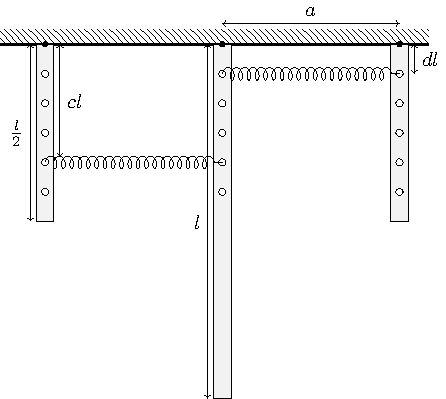
\includegraphics[width=0.8\linewidth]{./Figures/system-diagram.pdf}
  \caption{Esquema de los p\'endulos en equilibrio. La distancia
  entre los ejes de rotaci\'on es $a$.}
  \label{fig:esquema_equilibrio}
\end{figure}

Las ecuaciones de movimiento del sistema se obtienen mediante la
aplicaci\'on de la sumatoria de torques, considerando tanto las
contribuciones de los resortes como la de la fuerza gravitacional
. Si bien los formalismos Lagrangiano y Hamiltoniano
ofrecen un enfoque m\'as general y elegante para sistemas complejos,
para el presente sistema de p\'endulos, la aplicaci\'on directa de
la segunda ley de Newton para rotaci\'on (sumatoria de torques)
resulta en un m\'etodo igualmente riguroso y conceptualmente claro
para la derivaci\'on de las ecuaciones de movimiento.
Es necesario, entonces, encontrar una expresi\'on para el torque
gravitacional en funci\'on de cualquier \'angulo $\theta_i$, as\'i
como una expresi\'on para las distancias del tipo $x_0 + \Delta x$,
que representan la elongaci\'on de los resortes en funci\'on de los
\'angulos $\theta_i$ y $\theta_{i\pm 1}$. Las barras se
enumeran de izquierda a derecha como 1, 2 y 3, seg\'un se muestra en la
\cref{fig:enumeracion_barras}.

\begin{figure}[htbp!]
  \centering
  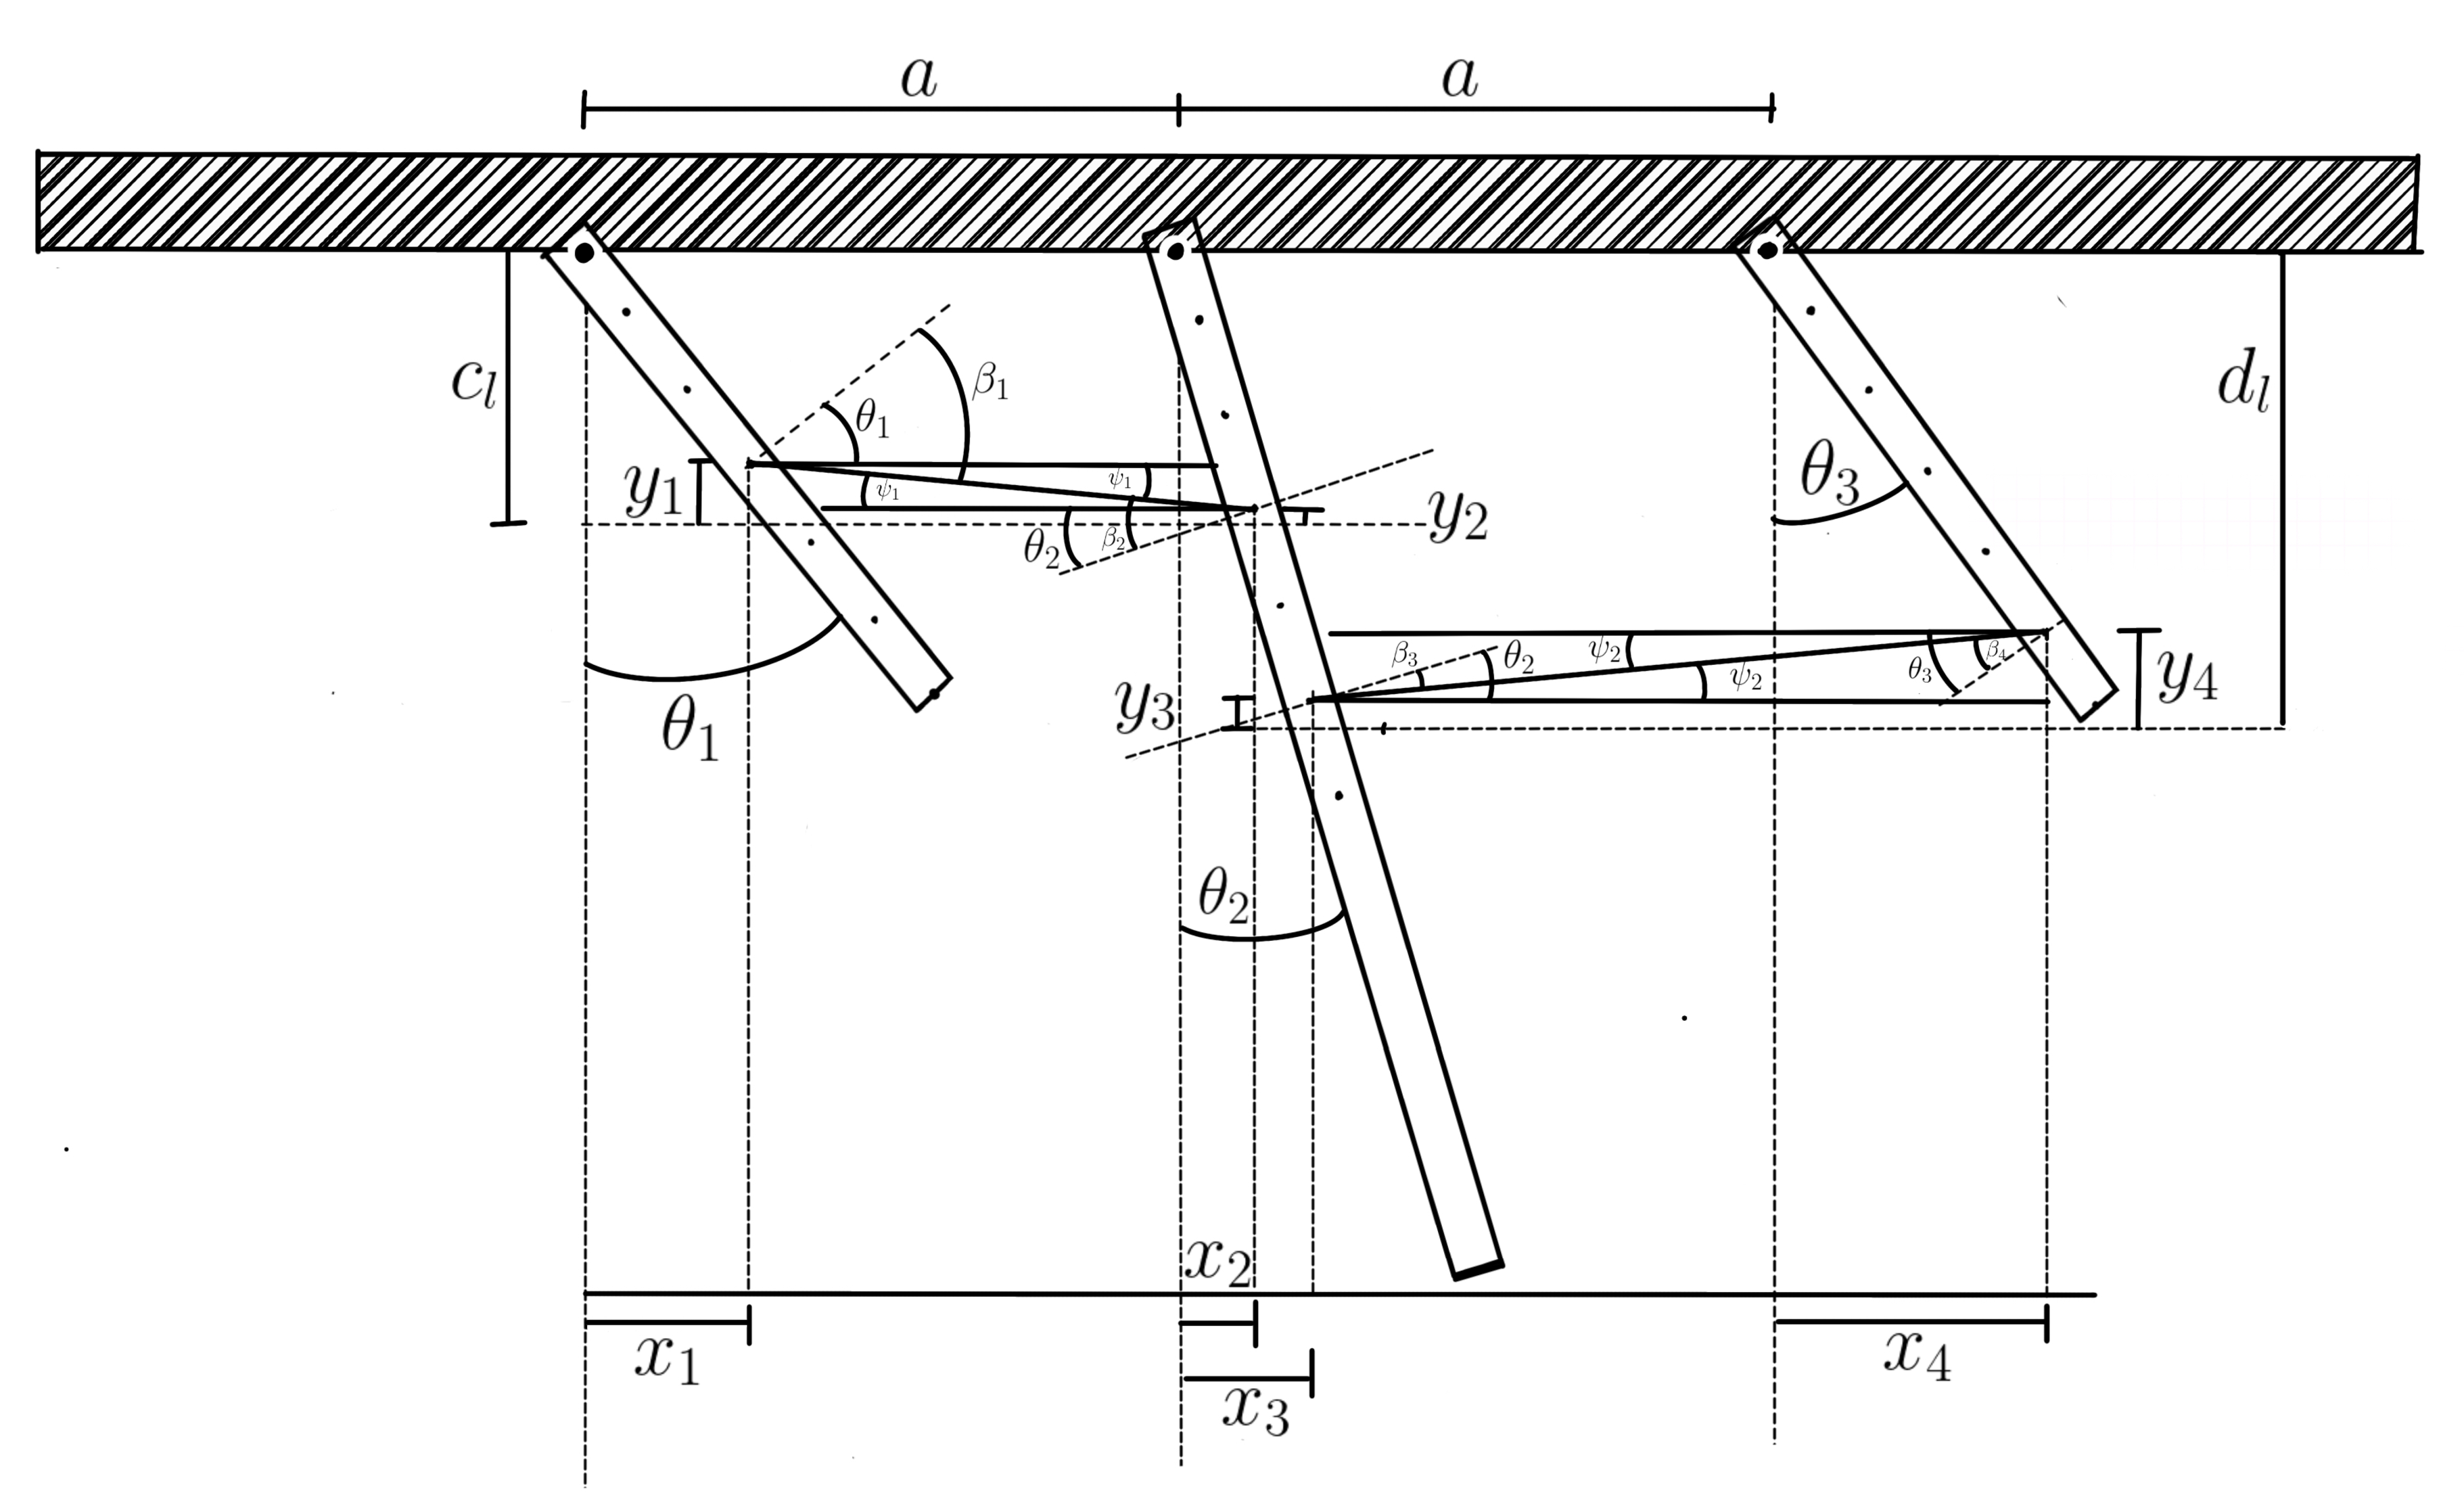
\includegraphics[width=0.8\linewidth]{Figures/Ilustración_sin_título 4.pdf}
  \caption{Numeraci\'on de las barras del sistema de p\'endulos:
  1 (izquierda), 2 (central), 3 (derecha).}
  \label{fig:enumeracion_barras}
\end{figure}

Al desplazar las barras 1 y 2 de su posici\'on de equilibrio, se
observa que la tangente de cada barra se desv\'ia un \'angulo
$\theta_i$ del eje horizontal. Esta condici\'on permite
construir un tri\'angulo rect\'angulo con las componentes $x_i$ e
$y_i$ de la posici\'on del punto de aplicaci\'on de la fuerza
el\'astica para cada barra, generalizada a cualquier fracci\'on de
la longitud $l$, tal como se ilustra en la \cref{fig:triangulo_posicion}.

\begin{figure}[htbp!]
  \centering
  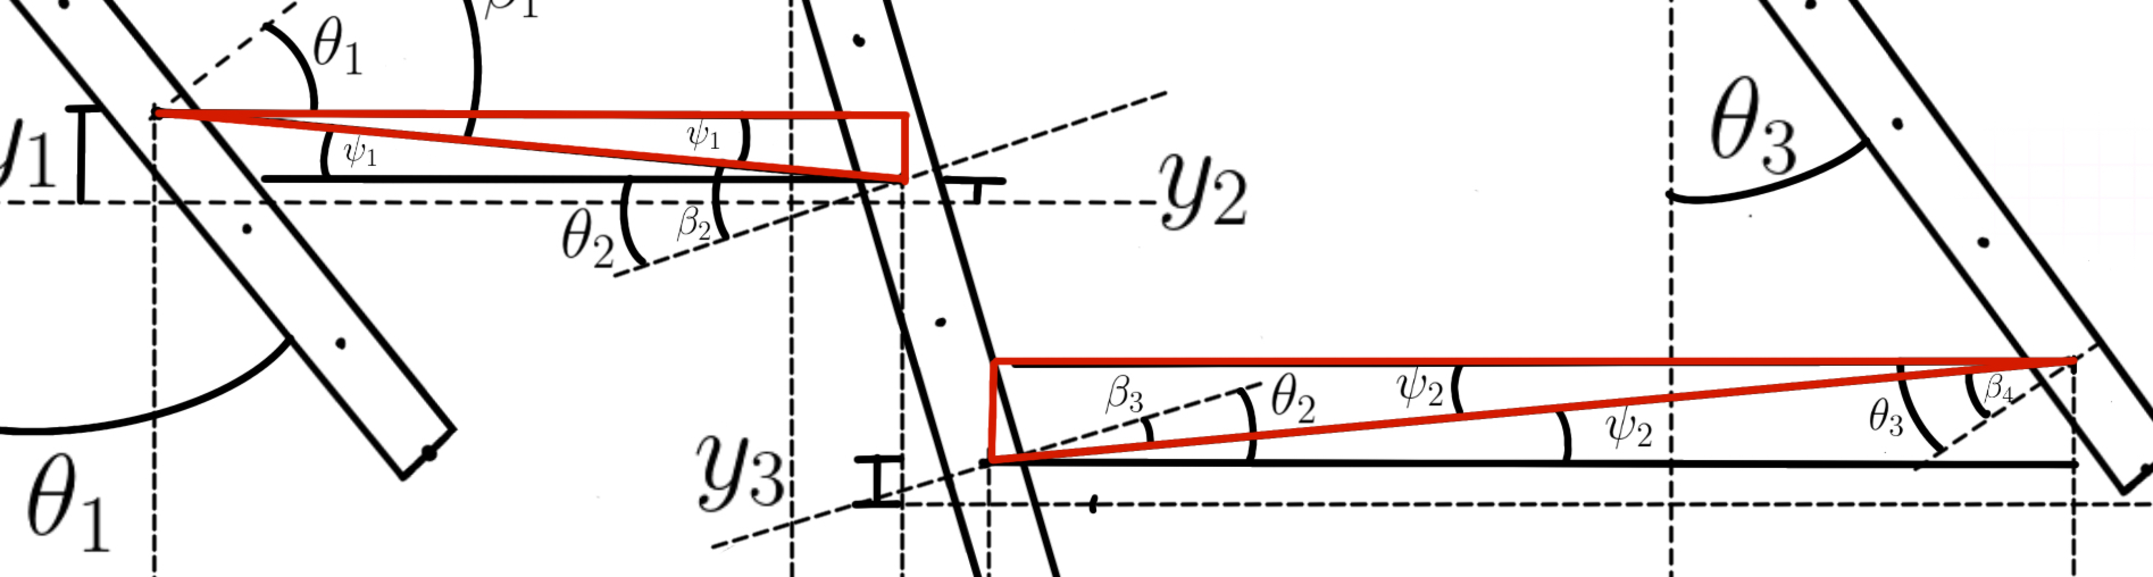
\includegraphics[width=0.8\linewidth]{Figures/Ilustración_sin_título 5.pdf}
  \caption{Construcci\'on geom\'etrica para determinar la posici\'on
  del punto de aplicaci\'on de la fuerza el\'astica en una barra.}
  \label{fig:triangulo_posicion}
\end{figure}

Las coordenadas $x_k$ e $y_k$ para $k = 1, 2$ est\'an definidas como:
\begin{align}
  x_k &= c l \sin(\theta_{k}) \label{eq:xk} \\
  y_k &= c l \cos(\theta_{k}) \label{eq:yk}
\end{align}
donde $c$ y $d$ son fracciones de la longitud de la barra $l$ que
indican la posici\'on de los puntos de acople de los resortes.
El tri\'angulo resultante est\'a definido por un \'angulo $\psi_1$,
el cual cumple la relaci\'on $\beta_1 + \psi_1 = \theta_1$, donde
$\beta_1$ corresponde al \'angulo entre la tangente de la barra 1 y
la l\'inea recta que conecta los puntos de aplicaci\'on.
A partir de este tri\'angulo, se obtiene la expresi\'on para la
elongaci\'on del resorte entre las barras 1 y 2:
\begin{equation}
  x_{01} + \Delta x_{1} = \sqrt{(y_2 - y_1)^2 + (a + x_2 - x_1)^2}
  \label{eq:elongacion1}
\end{equation}
con $x_{01}$ como la longitud natural del resorte.
Y el \'angulo $\psi_1$ est\'a dado por:
\begin{equation}
  \psi_1 = \arctan\left( \frac{y_2 - y_1}{a - x_1 + x_2} \right)
  \label{eq:psi1}
\end{equation}
De forma an\'aloga, para el resorte entre las barras 2 y 3, se
utiliza un punto de aplicaci\'on $d l$, resultando en:
\begin{align}
  \psi_2 &= \arctan \left( \frac{y_4 - y_3}{a - x_3 + x_4} \right) \label{eq:psi2}, \\
  x_{02} + \Delta x_{2} &= \sqrt{(y_4 - y_3)^2 + (a + x_4 - x_3)^2} \label{eq:elongacion2}
\end{align}
Donde para $j = 3, 4$, las coordenadas $x_j$ e $y_j$ son:
\begin{align}
  x_j &= d l \sin(\theta_{j}) \label{eq:xj} \\
  y_j &= d l \cos(\theta_{j}) \label{eq:yj}
\end{align}
El torque gravitacional sobre cada barra $i$ est\'a dado por:
\begin{equation}
  \tau_{g_i} = y_{\text{cm}_i} \, m_i \, g \sin(\theta_i) \label{eq:tau_g}
\end{equation}
Donde $y_{\text{cm}_i}$ es la posici\'on del centro de masa de la
barra $i$. Para los torques el\'asticos, se deben
considerar los \'angulos $\beta_i$, definidos como:
\begin{align}
  \beta_1 + \psi_1 &= \theta_1, & \beta_2 + \psi_1 &= \theta_2, \label{eq:beta1_psi1}\\
  \beta_3 + \psi_2 &= \theta_2, & \beta_4 + \psi_2 &= \theta_3 \label{eq:beta3_psi2}
\end{align}
Es importante notar que, debido a las distintas posiciones de
aplicaci\'on de los resortes entre los pares de barras, aparecen
cuatro \'angulos $\beta_i$, donde los \'indices 2 y 3 se refieren
a la barra central. La sumatoria de torques para cada
p\'endulo, considerando el sentido antihorario como positivo, resulta
en las siguientes ecuaciones de movimiento:
\begin{align}
  \sum \tau_{m_1} &= c l k_1 (\Delta x_1) \cos(\beta_1) - m_1 g y_{\text{cm}_1} \sin(\theta_1) = I_1 \, \ddot{\theta}_1 \label{eq:tau_m1}, \\
  \sum \tau_{m_2} &= d l k_2 (\Delta x_2) \cos(\beta_3) - c l k_1 (\Delta x_1) \cos(\beta_2) - m_2 g y_{\text{cm}_2} \sin(\theta_2) = I_2 \, \ddot{\theta}_2 \label{eq:tau_m2}, \\
  \sum \tau_{m_3} &= -d l k_2 (\Delta x_2) \cos(\beta_4) + m_3 g y_{\text{cm}_3} \sin(\theta_3) = I_3 \, \ddot{\theta}_3 \label{eq:tau_m3}
\end{align}

\subsection*{Aproximaciones para \'Angulos Peque\~nos}

Con el fin de obtener una soluci\'on anal\'itica aproximada que permita
calcular las frecuencias naturales del sistema, se aplican
las siguientes aproximaciones para \'angulos peque\~nos ($\theta \ll 1$ rad):
\begin{align*}
  \sin(\theta) &\approx \theta, \\
  \cos(\theta) &\approx 1, \\
  \tan(\theta) &\approx \theta.
\end{align*}
Aplicando estas aproximaciones, las coordenadas $x_k$ e $y_k$ se
simplifican a:
\begin{align*}
  x_1 &= c l \theta_1, & x_2 &= c l \theta_2 \\
  x_3 &= d l \theta_2, & x_4 &= d l \theta_3 \\
  y_1 &= c l, & y_2 &= c l \\
  y_3 &= d l, & y_4 &= d l
\end{align*}
Si se cumple la condici\'on de que las longitudes naturales de los
resortes son iguales a la separaci\'on entre los ejes, es decir,
$x_{01} = x_{02} = a$, las elongaciones de los resortes $\Delta x_1$
y $\Delta x_2$ se simplifican a:
\begin{align}
  \Delta x_1 &= cl(\theta_2 - \theta_1) \label{eq:deltax1_approx}, \\
  \Delta x_2 &= dl(\theta_3 - \theta_2) \label{eq:deltax2_approx}.
\end{align}
Adem\'as, si se asume que $\arctan(\psi_i) \approx \psi_i \approx 0$,
lo que implica que la fuerza el\'astica act\'ua aproximadamente en
la direcci\'on horizontal, entonces los \'angulos $\beta_i$ se
aproximan a los \'angulos $\theta_i$ ($\beta_i \approx \theta_i$).
Esto simplifica la sumatoria de torques a:
\begin{align}
  I_1 \ddot{\theta}_1 &= (cl)^2 k_1 (\theta_2 - \theta_1) - m_1 g y_{\text{cm}_1} \theta_1 \label{eq:eq_mov_lin1}, \\
  I_2 \ddot{\theta}_2 &= (dl)^2 k_2 (\theta_3 - \theta_2) - (cl)^2 k_1 (\theta_2 - \theta_1) - m_2 g y_{\text{cm}_2} \theta_2 \label{eq:eq_mov_lin2}, \\
  I_3 \ddot{\theta}_3 &= -(dl)^2 k_2 (\theta_3 - \theta_2) - m_3 g y_{\text{cm}_3} \theta_3 \label{eq:eq_mov_lin3}.
\end{align}
Finalmente, el sistema de ecuaciones diferenciales lineales queda
expresado como:
\begin{align}
  \ddot{\theta}_1 &=\; -\theta_1 \left( \frac{(cl)^2 k_{1} + y_{\text{cm}_1} m_1 g}{I_1} \right) + \theta_2 \left( \frac{k_1 (cl)^2}{I_1} \right) \label{eq:eom1} \\
  \ddot{\theta}_2 &=\; \theta_1 \left( \frac{k_1 (cl)^2}{I_2} \right) - \theta_2 \left( \frac{k_2 (dl)^2 + k_1 (cl)^2 + y_{\text{cm}_2} m_2 g}{I_2} \right) + \theta_3 \left( \frac{k_2 (dl)^2}{I_2} \right) \label{eq:eom2} \\
  \ddot{\theta}_3 &=\; \theta_2 \left( \frac{k_2 (dl)^2}{I_3} \right) - \theta_3 \left( \frac{k_2 (dl)^2 + y_{\text{cm}_3} m_3 g}{I_3} \right) \label{eq:eom3}
\end{align}
Estas ecuaciones forman un sistema lineal de ecuaciones
diferenciales ordinarias acopladas, que pueden ser presentadas
como una ecuaci\'on matricial \cref{eq:matrix-form} donde
$\bm{M}$, $\bm{K}$ y $\bm{\Theta}$ representan una matriz cuadrada
diagonal con los t\'erminos de inercia, una matriz cuadrada con los
t\'erminos de acople, y un vector columna con las coordenadas
angulares, respectivamente.
\begin{equation}
  \mathbf{M} \ddot{\bm{\Theta}} + \mathbf{K} \bm{\Theta} = \mathbf{0}
  \label{eq:matrix-form}
\end{equation}
Este sistema linealizado permite determinar las frecuencias
naturales del sistema al resolver el problema de valores propios
asociado.

\subsection*{Modos Normales}

A partir de la ecuaci\'on en forma matricial \cref{eq:matrix-form} se
lleva a un problema de valores propios para determinar los modos
normales. Esto se logra con la posibilidad de invertir la matriz con
los t\'erminos inerciales e identificar la segunda derivada como el
operador:
\begin{equation}
  \mathbf{D}^2_t \bm{\Theta} = - \mathbf{\Omega} \bm{\Theta}
  \label{eq:eigenproblem}
\end{equation}
donde $\mathbf{D}^2_t$ representa el operador de la segunda derivada
temporal y $\mathbf{\Omega} = \mathbf{M}^{-1}\mathbf{K}$ es la matriz
din\'amica del sistema. Dada la complejidad del c\'alculo anal\'itico
para un sistema de tres grados de libertad, se emplea una soluci\'on
num\'erica usando la librer\'ia de Python SciPy para determinar
las frecuencias de los modos normales y sus correspondientes vectores
propios.

\section{Metodolog\'ia Experimental}

La metodolog\'ia experimental se estructur\'o en varias etapas
fundamentales: dise\~no y construcci\'on del montaje,
caracterizaci\'on de sus componentes y adquisici\'on de datos
mediante sensores angulares.

\subsection*{Construcci\'on del Montaje}

Para la construcci\'on del sistema se utilizaron tres barras
met\'alicas de alta densidad, lo que contribuye a la rigidez del
sistema y a una mejor definici\'on de su centro de masa.
Las barras laterales tienen una longitud de
$l/2 = \qty{28.0(1)}{\centi\metre}$, mientras que la barra central
posee una longitud de $l = \qty{56.0(1)}{\centi\metre}$.
Las masas y las posiciones de los centros de masa de cada barra
fueron determinadas experimentalmente y se resumen en el
\cref{tab:bars-dat}. La posici\'on del centro de masa,
$y_{\text{cm}_i}$, se mide desde el punto de pivote de cada p\'endulo.

\begin{table*}[htbp!]
  \caption{Parámetros físicos de las barras empleadas en el montaje.
    La incertidumbre para la posición del centro de masa (\(y_{\text{cm}_i}\)) es
    de \qty{0.1}{\centi\metre} y para la masa (\(m_i\)) es de \qty{0.1}{\gram}.
  }
  \centering
  \pgfplotstabletypeset[
  col sep=comma,
  zerofill,
  columns/i/.style={
    string type,
    column type={c},
    column name={\(i\)},
  },
  columns/y_cm_i/.style={
    column name={\(y_{\text{cm}_i} [\si{\centi\metre}]\)},
    precision=1,
    fixed,
    fixed zerofill,
  },
  columns/m_i/.style={
    column type={c},
    column name={\(m_i [\si{\gram}]\)},
    dec sep align,
    precision=1,
    fixed,
    fixed zerofill,
  },
  every head row/.style={
    before row=\toprule,
    after row=\midrule,
  },
  every last row/.style={
    after row=\bottomrule,
  }
  ]\mydata
  \label{tab:bars-dat}
\end{table*}

Las barras fueron perforadas en m\'ultiples puntos para permitir
diversas configuraciones de acople de los resortes. La
\cref{fig:barras} muestra las barras met\'alicas preparadas para el
montaje.

\begin{figure}[htbp!]
  \centering
  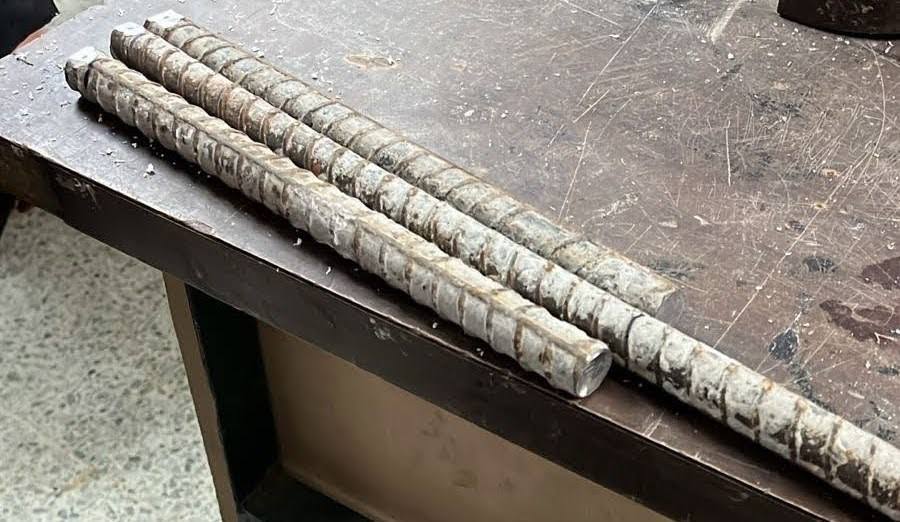
\includegraphics[width=0.6\linewidth]{Figures/metal-bars.jpeg}
  \caption{Barras met\'alicas preparadas para el montaje de los
  p\'endulos, mostrando las perforaciones para el acople de resortes.}
  \label{fig:barras}
\end{figure}

\subsection*{Medici\'on de la Constante El\'astica}

La constante el\'astica de los resortes empleados ($k_1$ y $k_2$) se
determin\'o experimentalmente. Se aplicaron masas conocidas a cada
resorte y se registraron los desplazamientos resultantes.
Mediante una regresi\'on lineal de los datos de fuerza
(peso aplicado) versus elongaci\'on, se obtuvieron los siguientes
valores para las constantes el\'asticas:
\begin{itemize}
  \item $k_1 = \qty{3.04(4)}{\N\per\m}$
  \item $k_2 = \qty{3.32(6)}{\N\per\m}$
\end{itemize}
El proceso gr\'afico de determinaci\'on de estas constantes se
ilustra en la \cref{fig:regresion}.

\begin{figure}[htbp!]
  \centering
  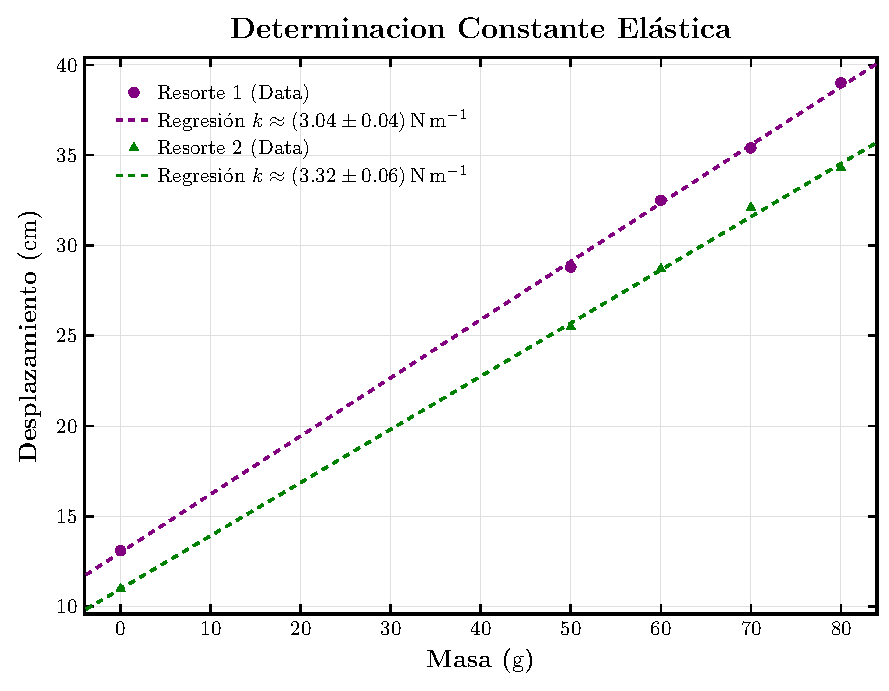
\includegraphics[width=0.75\linewidth]{Figures/springs-plot.pdf}
  \caption{Determinaci\'on de la constante el\'astica de los resortes
    mediante regresi\'on lineal de los datos de fuerza aplicada en
  funci\'on del desplazamiento.}
  \label{fig:regresion}
\end{figure}

\subsection*{Integraci\'on del Sistema de Medici\'on}

Para registrar los desplazamientos angulares $\theta_i(t)$ de
cada p\'endulo, se integraron sensores angulares rotacionales
(Cassy) en cada uno de los puntos de pivote. Las barras de los
p\'endulos se fijaron a las poleas de los sensores utilizando
alambre dulce. Aunque esta metodolog\'ia de fijaci\'on podr\'ia
introducir un m\'inimo juego mec\'anico, se realiz\'o con cautela
para minimizar cualquier holgura y asegurar mediciones angulares
precisas. La \cref{fig:montaje} presenta el montaje experimental
completo con los sensores integrados.

\begin{figure}[htbp!]
  \centering
  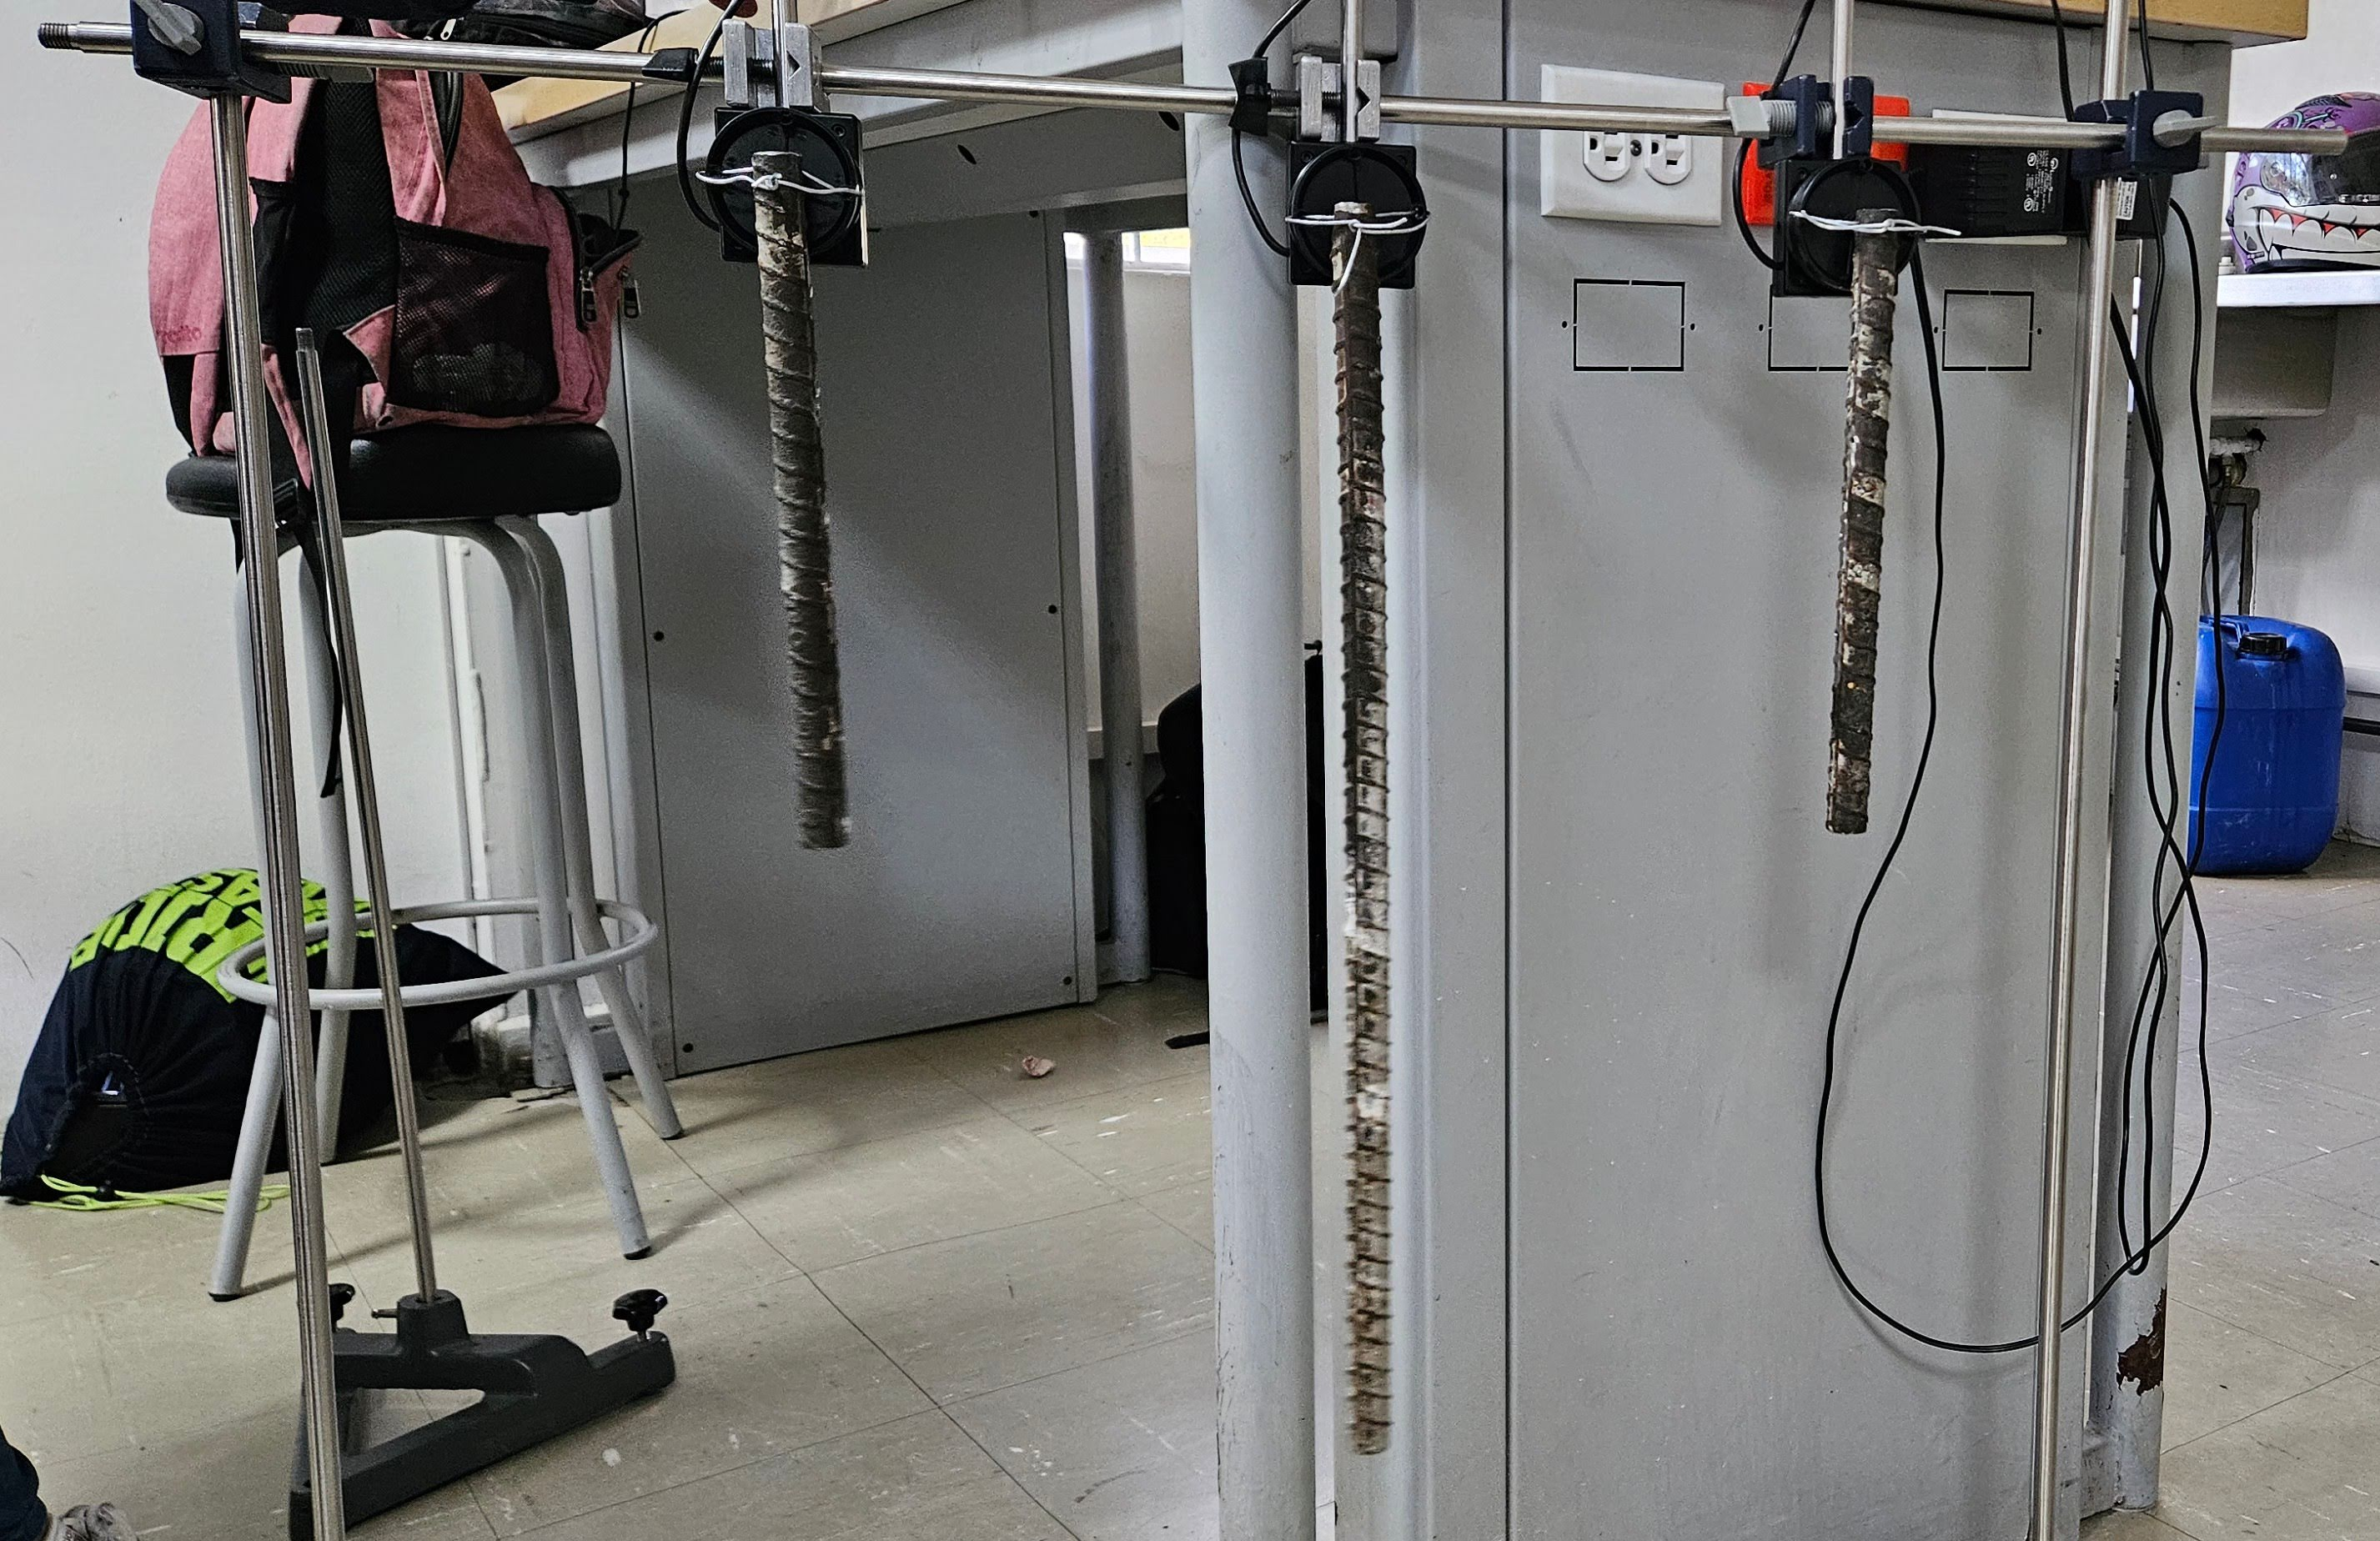
\includegraphics[width=0.75\textwidth]{Figures/set-up.jpeg}
  \caption{Montaje experimental completo del sistema de tres
    p\'endulos acoplados, con los sensores angulares Cassy
  integrados en los pivotes.}
  \label{fig:montaje}
\end{figure}

\subsection*{Toma de Datos y Configuraciones Experimentales}

Se realizaron mediciones bajo cinco configuraciones distintas de
acoplamiento de resortes, esquematizadas en la \cref{fig:configs}.
Para cada configuraci\'on, se investigaron tres tipos de
condiciones iniciales para excitar el sistema:
\begin{itemize}
  \item (001): Desplazamiento inicial \'unicamente del p\'endulo 3.
  \item (010): Desplazamiento inicial \'unicamente del p\'endulo 2.
  \item (101): Desplazamiento inicial sim\'etrico de los p\'endulos
    1 y 3 (en la misma direcci\'on y amplitud).
\end{itemize}
Cada medici\'on se registr\'o durante un intervalo aproximado de
\qty{30}{\second}, permitiendo la captura de m\'ultiples
oscilaciones completas. Los datos de los \'angulos en funci\'on
del tiempo fueron almacenados digitalmente para su posterior
an\'alisis y comparaci\'on con los resultados te\'oricos derivados
de los modos normales de oscilaci\'on.

\begin{figure}[htbp!]
  \centering
  \subfloat[Configuraci\'on 1-5\label{fig:conf-1-5}]{
    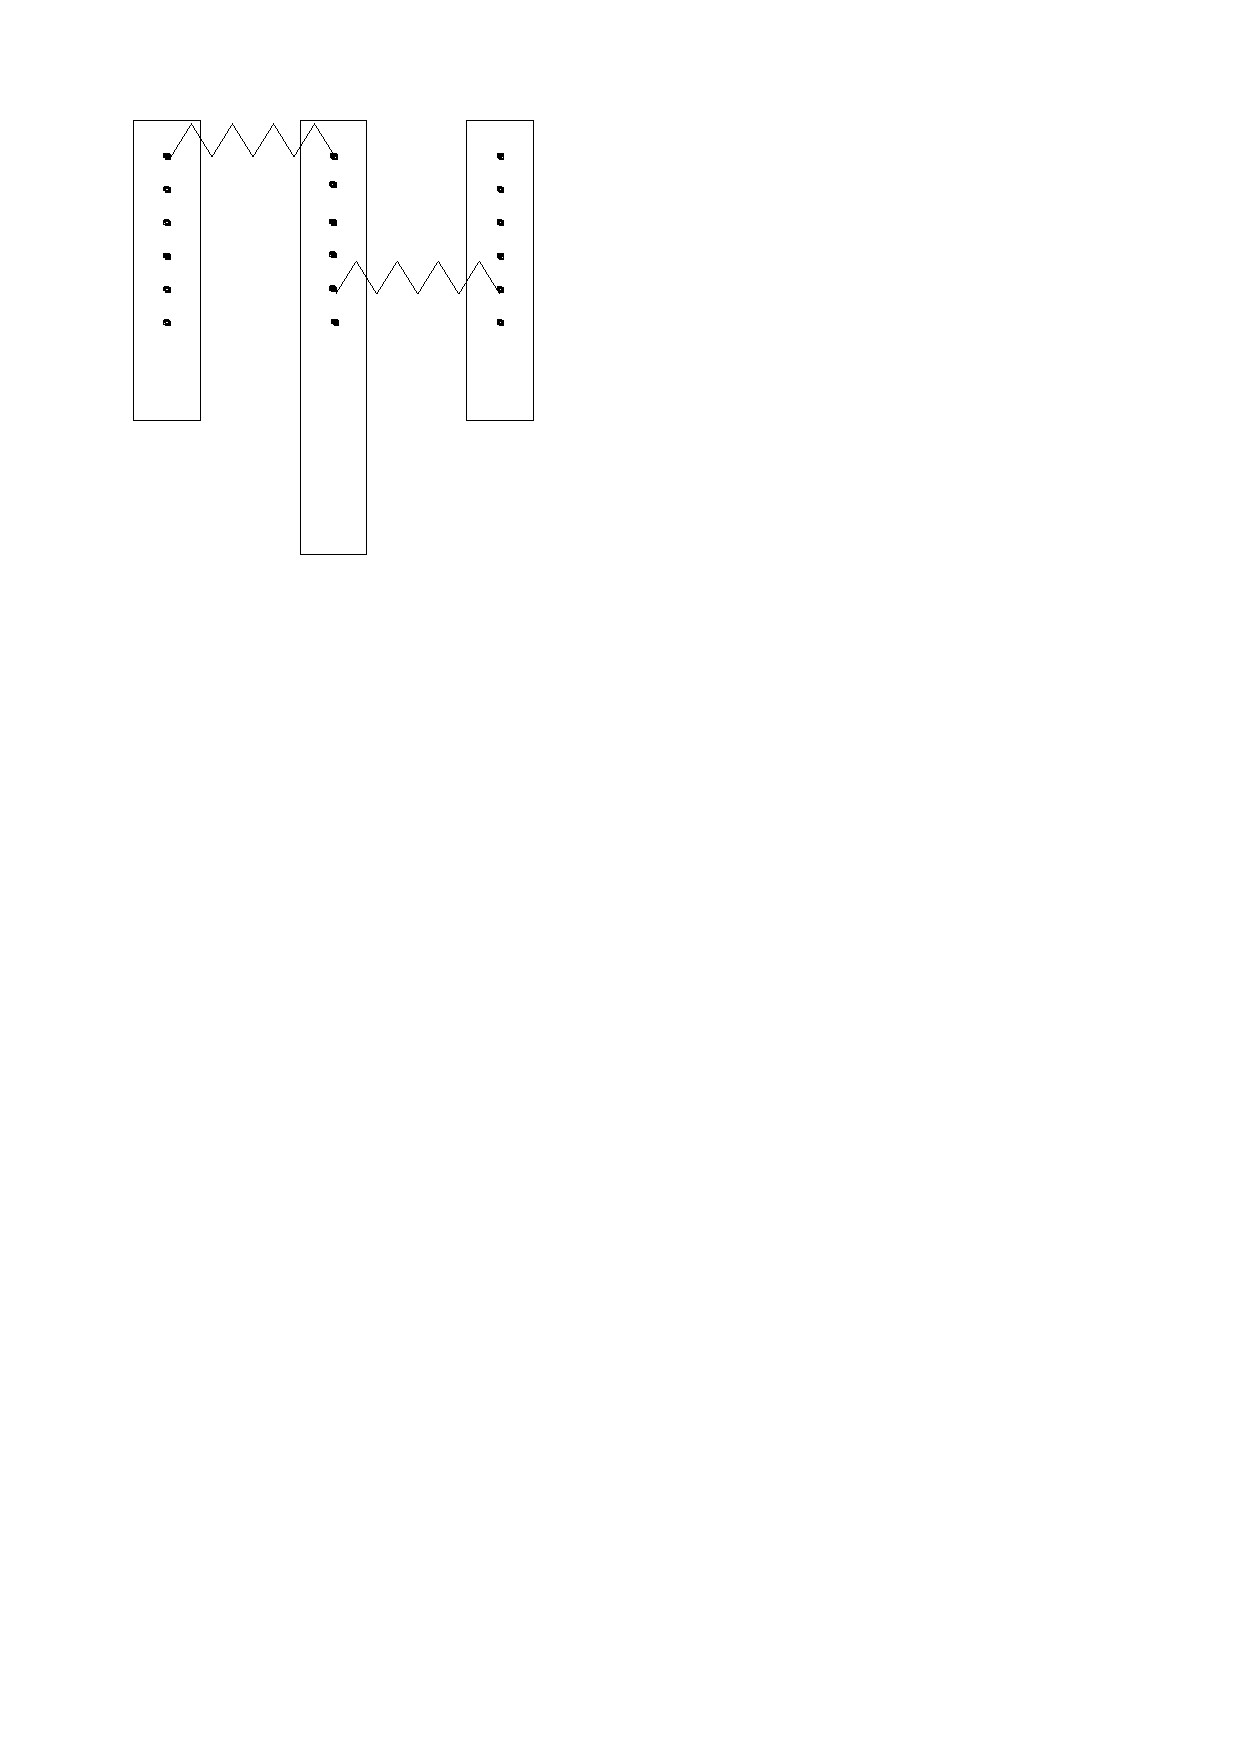
\includegraphics[width=0.3\textwidth]{./Figures/15.pdf}
  }
  \hfill
  \subfloat[Configuraci\'on 1-6\label{fig:conf-1-6}]{
    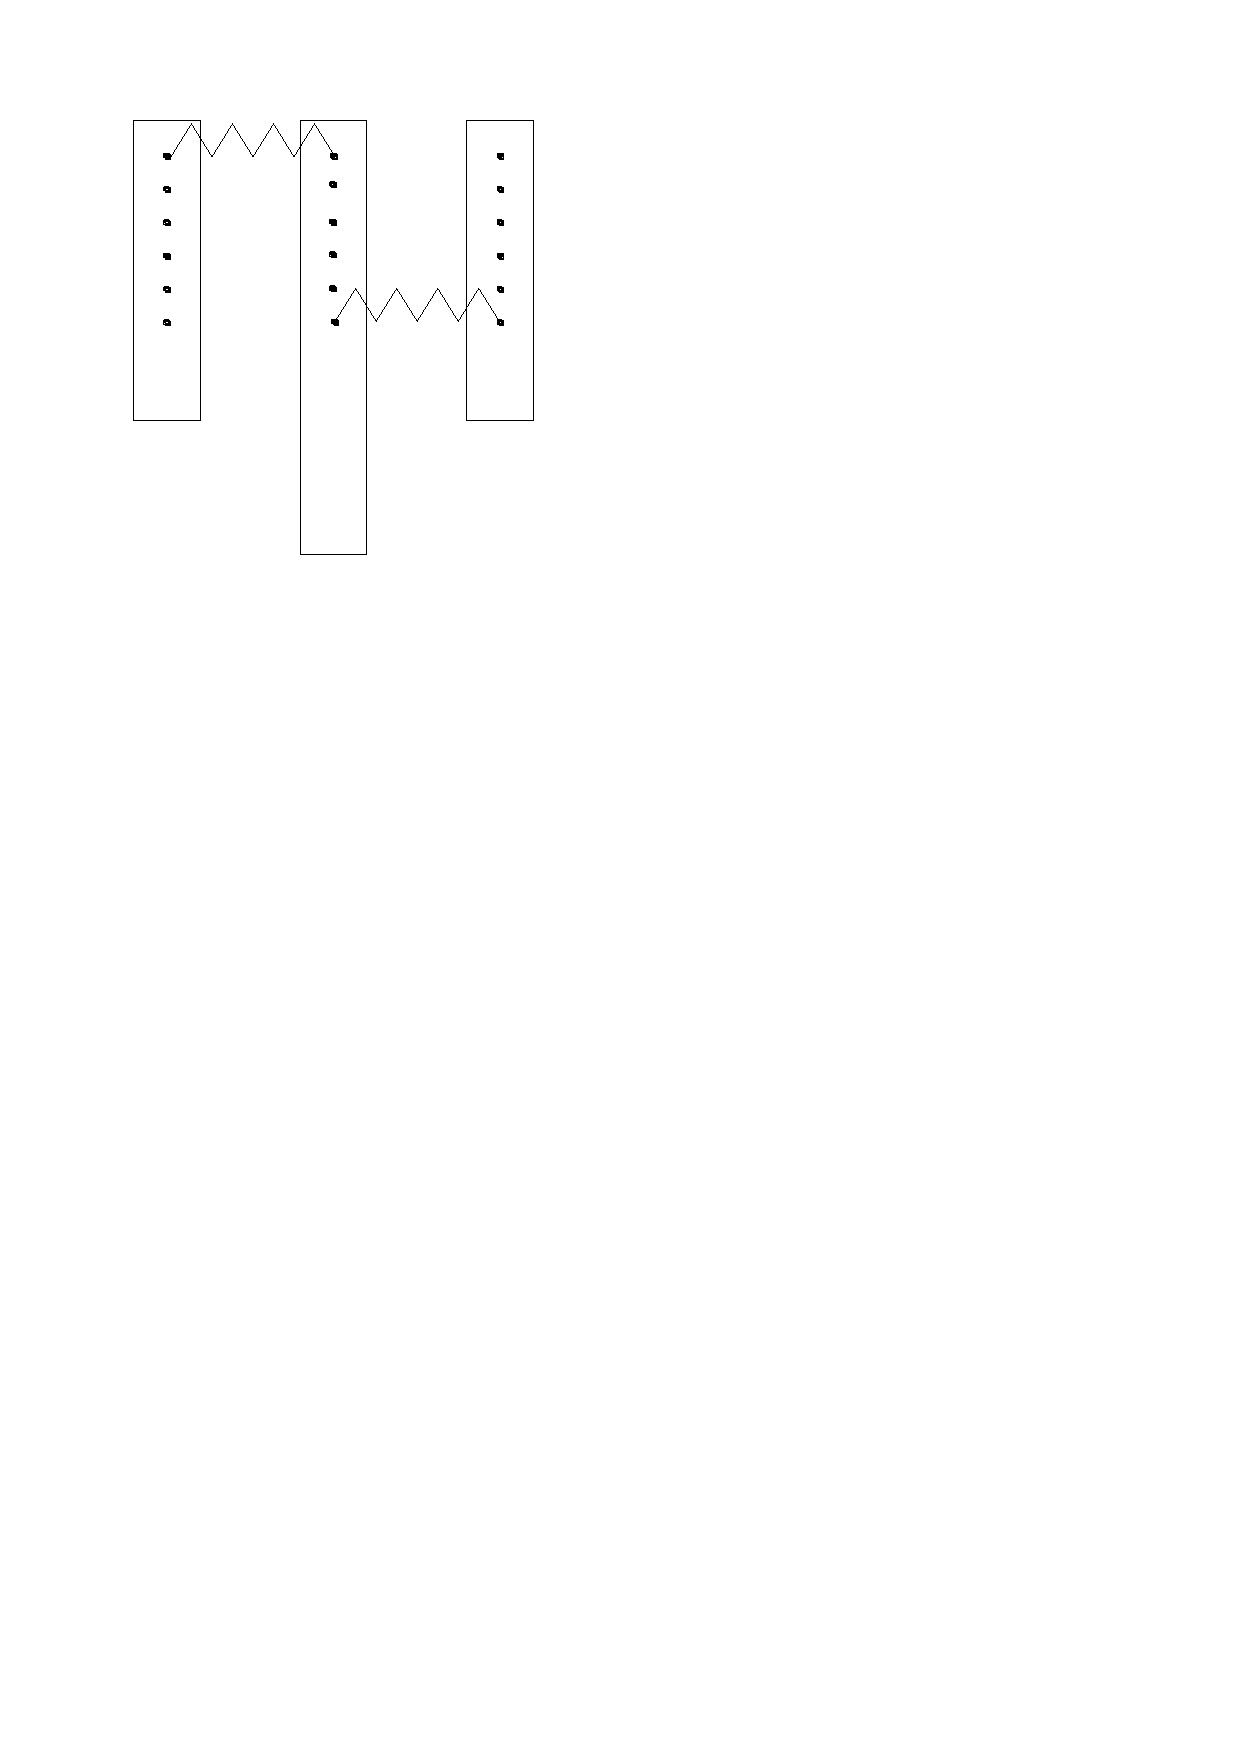
\includegraphics[width=0.3\textwidth]{./Figures/16.pdf}
  }
  \hfill
  \subfloat[Configuraci\'on 2-6\label{fig:conf-2-6}]{
    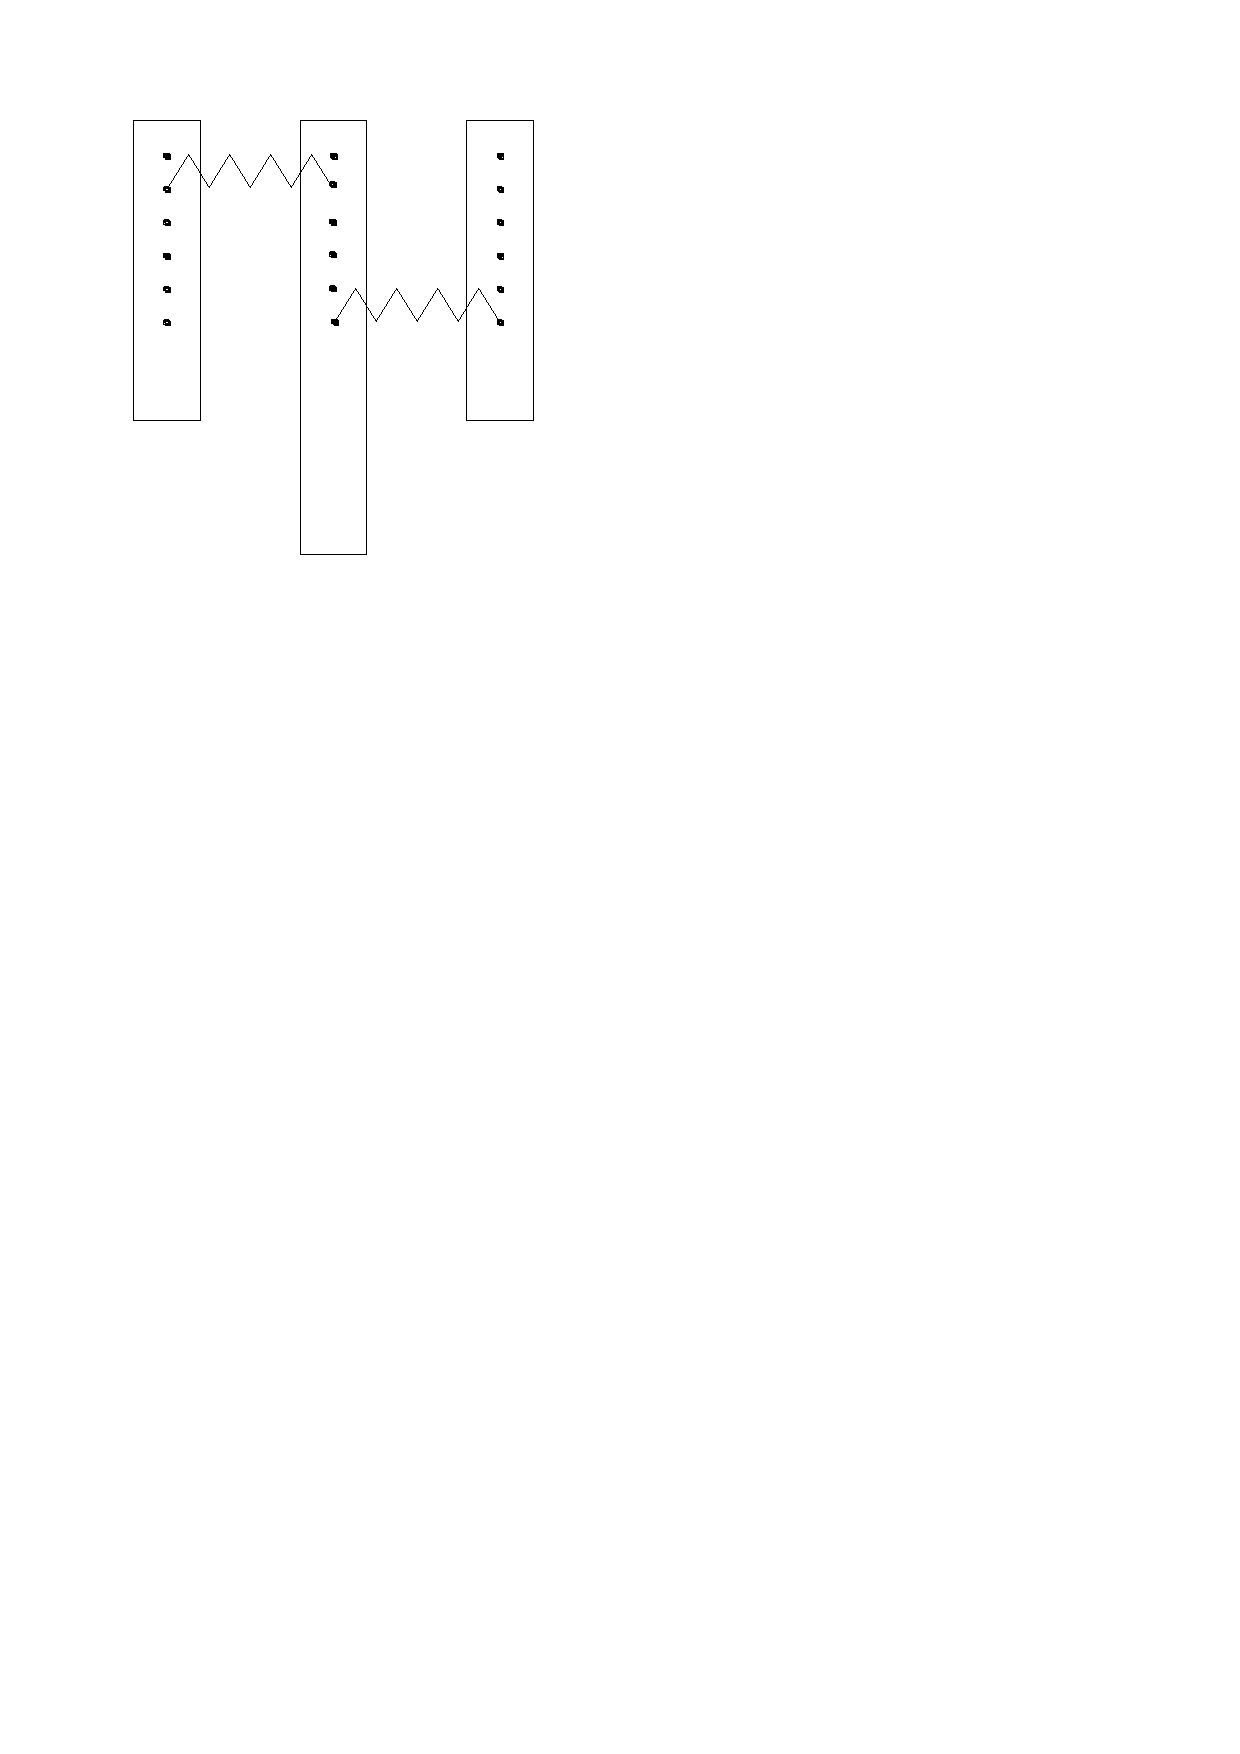
\includegraphics[width=0.3\textwidth]{./Figures/26.pdf}
  }

  \vspace{0.5cm}

  \subfloat[Configuraci\'on 4-6\label{fig:conf-4-6}]{
    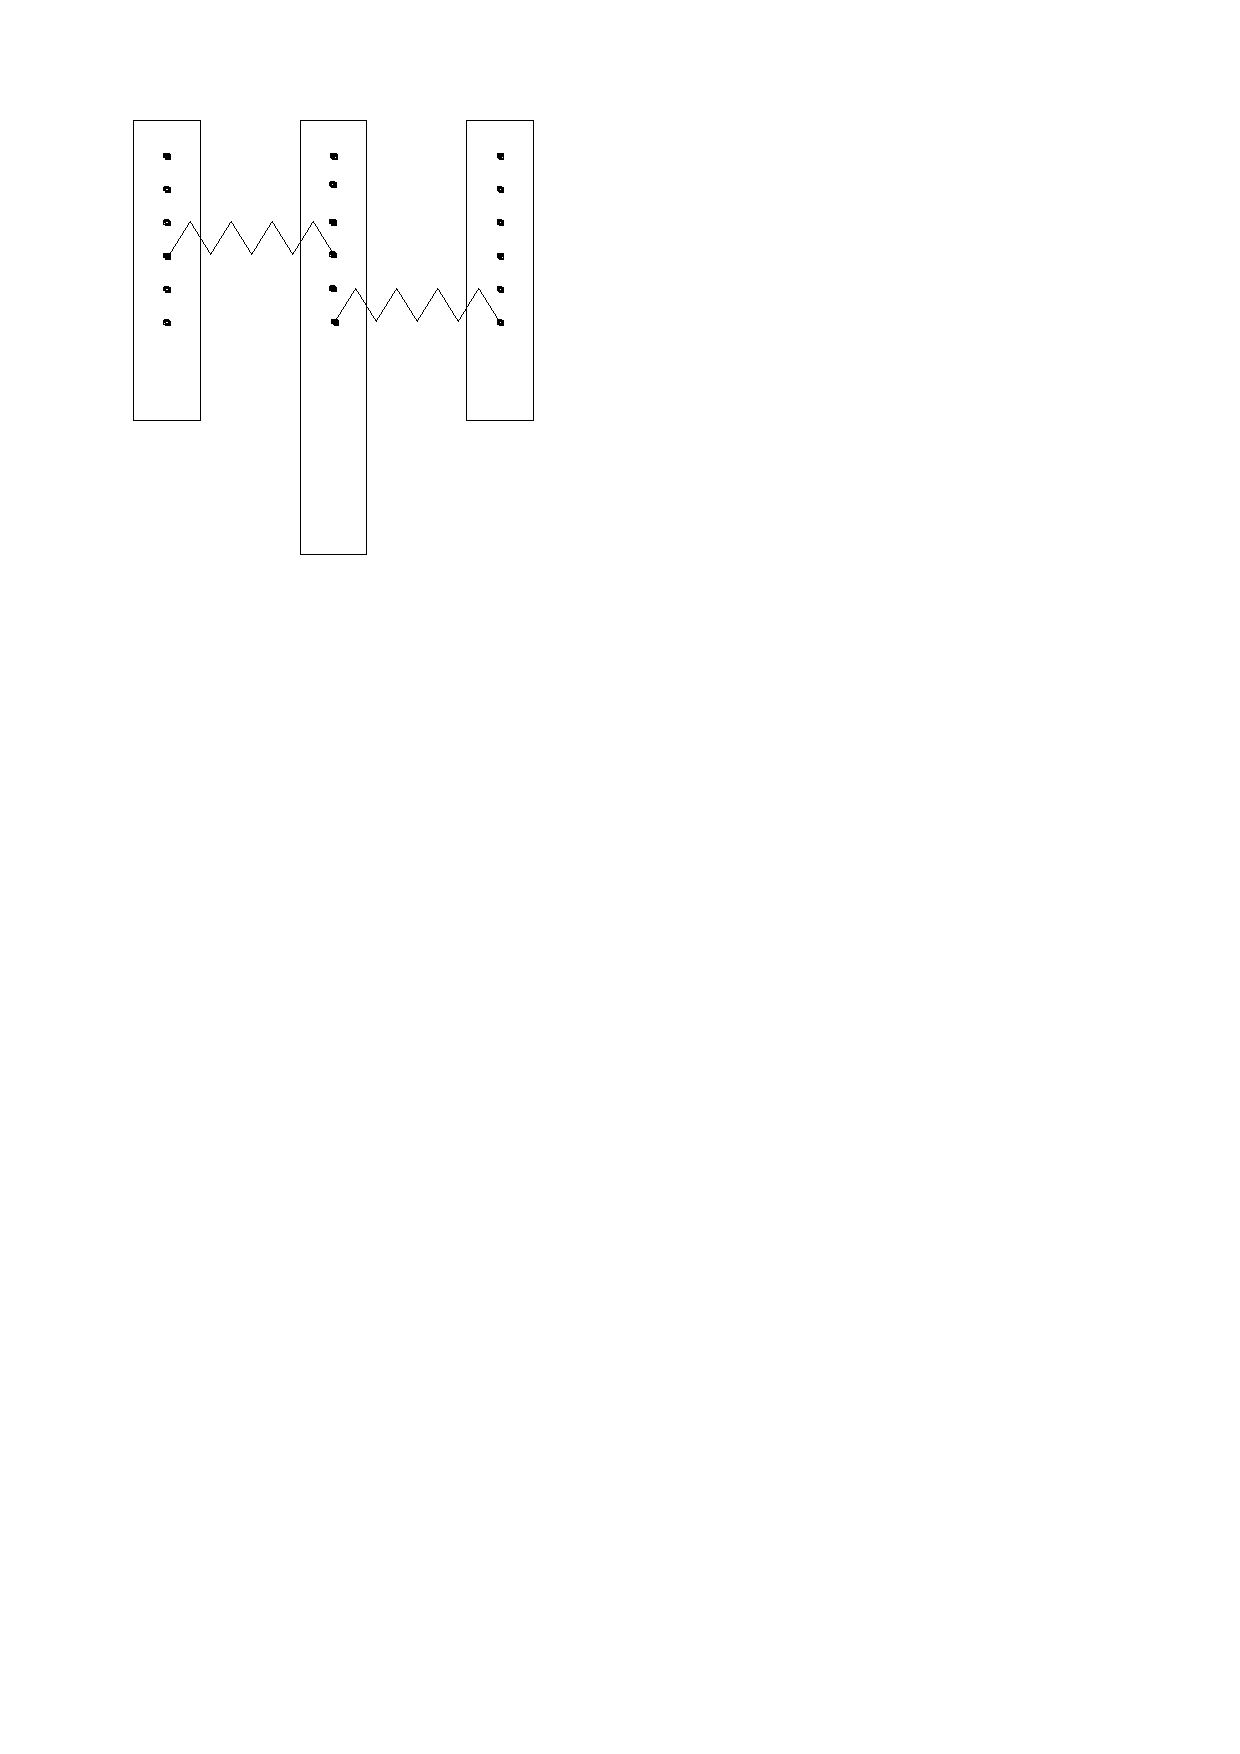
\includegraphics[width=0.3\textwidth]{./Figures/46.pdf}
  }
  \hspace{0.1\textwidth}
  \subfloat[Configuraci\'on 6-6\label{fig:conf-6-6}]{
    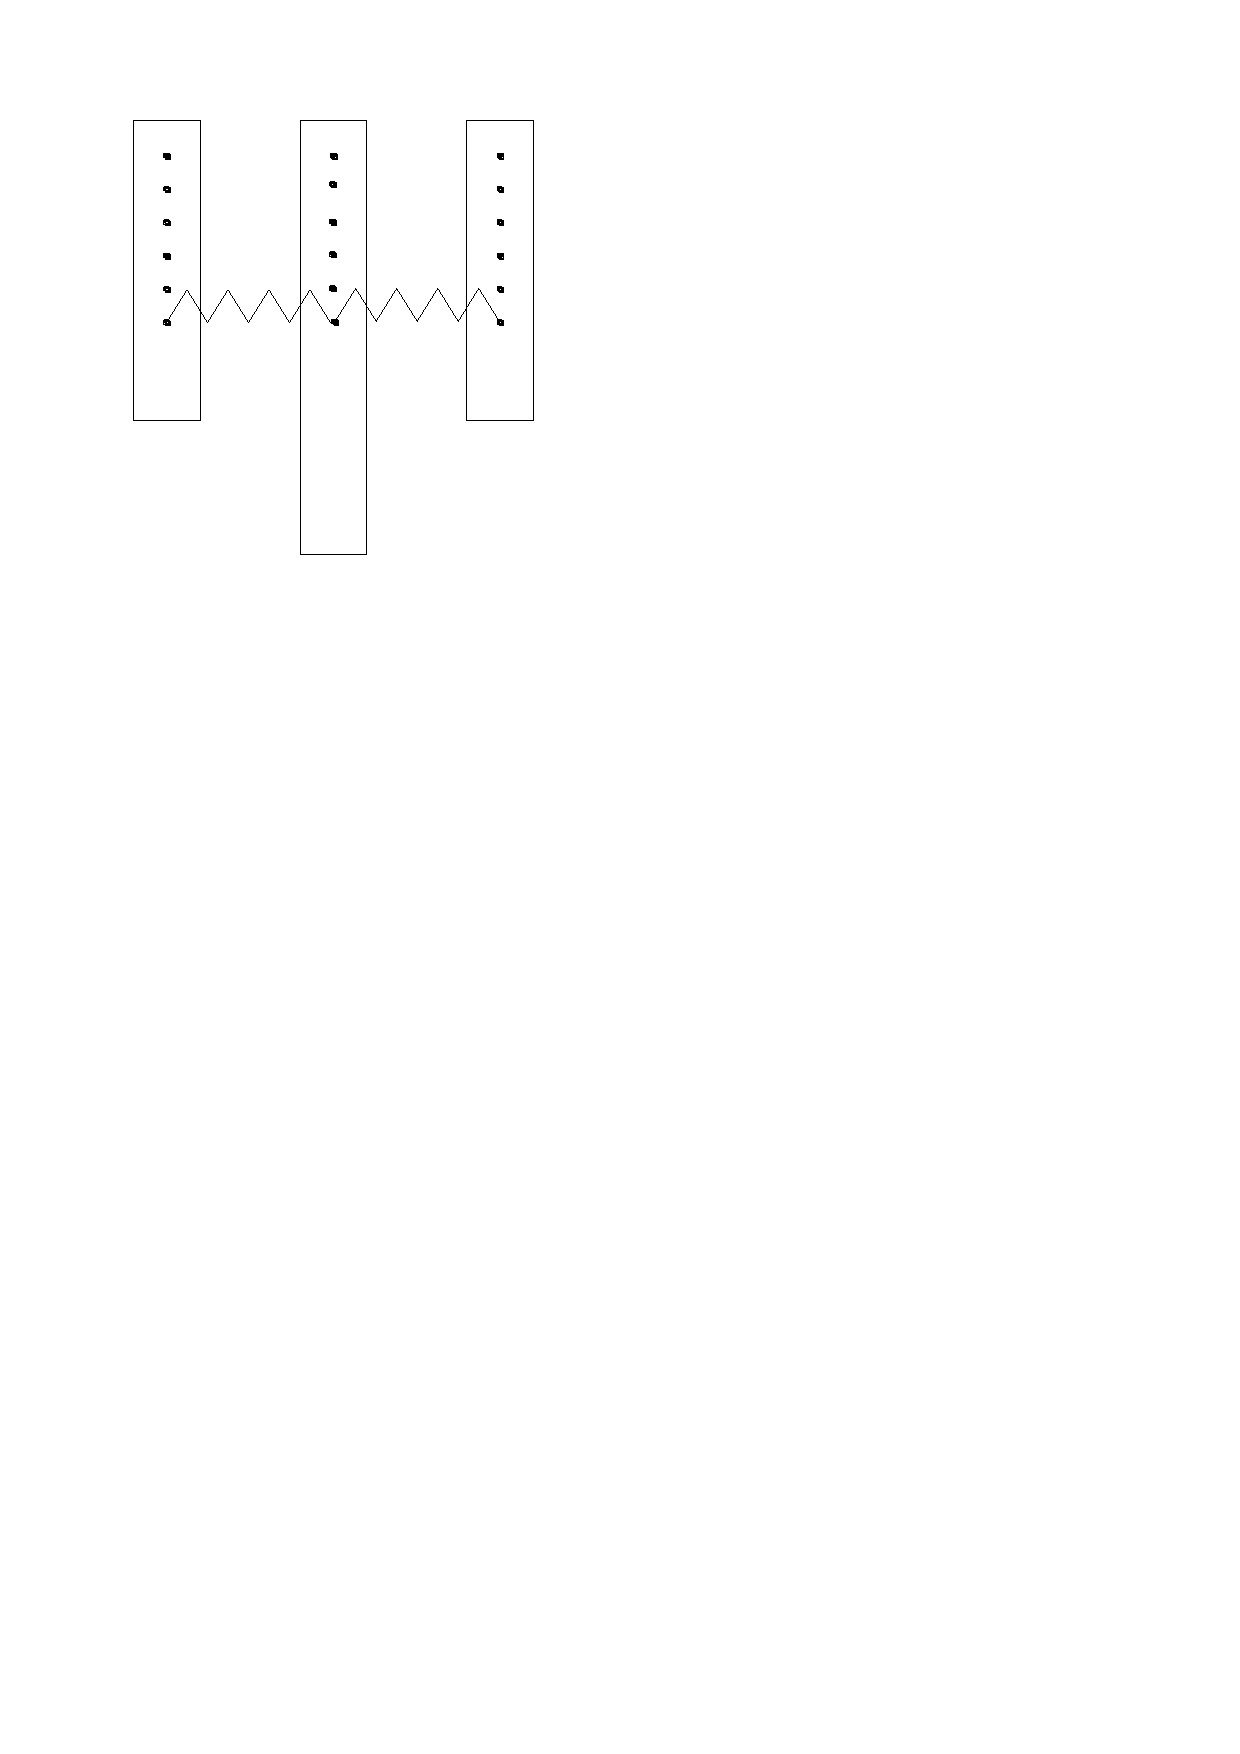
\includegraphics[width=0.3\textwidth]{./Figures/66.pdf}
  }
  \caption{Representaci\'on esquem\'atica de las cinco configuraciones de
    acoplamiento de resortes estudiadas. La nomenclatura 'X-Y' en
    cada subfigura (e.g., 1-5) indica los orificios espec\'ificos
    (numerados) en los p\'endulos adyacentes donde se anclaron
  los extremos de los resortes.}
  \label{fig:configs}
\end{figure}

\subsection*{Fundamento Te\'orico del An\'alisis Espectral}

El movimiento de un sistema lineal (o linealizado, como en la
aproximaci\'on de peque\~nas oscilaciones) con m\'ultiples grados de
libertad puede describirse como una superposici\'on de sus
modos normales de oscilaci\'on. Cada modo normal es un patr\'on de
movimiento colectivo en el que todas las partes del sistema oscilan
sinusoidalmente con la misma frecuencia caracter\'istica y una fase
relativa constante. Estas frecuencias son propiedades intr\'insecas
del sistema, determinadas por sus par\'ametros f\'isicos (masas,
longitudes, constantes de acoplamiento, etc.).

El Teorema de Fourier establece que cualquier se\~nal
peri\'odica (o una se\~nal de duraci\'on finita, como los datos
experimentales) puede representarse como una suma de funciones
sinusoidales (senos y cosenos) de diferentes frecuencias,
amplitudes y fases. La Transformada de Fourier es la
herramienta matem\'atica que formaliza esta descomposici\'on,
mapeando la se\~nal del dominio del tiempo al dominio de la
frecuencia. Al aplicar la Transformada de Fourier a una se\~nal de
movimiento como $\theta(t)$, se obtiene su espectro de
frecuencias, el cual revela la ``cantidad'' (amplitud o potencia)
de cada componente frecuencial presente en la se\~nal original \cite{Stein2003}.

Cuando el sistema de p\'endulos acoplados oscila, su movimiento
angular $\theta_i(t)$ es, en esencia, una mezcla de las
oscilaciones de sus modos normales. Por lo tanto, las frecuencias
que aparecen con mayor amplitud en el espectro de Fourier de
$\theta_i(t)$ corresponden directamente a las frecuencias
naturales de estos modos normales. La Transformada R\'apida de
Fourier (FFT) es simplemente un algoritmo computacionalmente
eficiente para calcular la Transformada Discreta de Fourier (DFT)
de una se\~nal muestreada digitalmente, como la obtenida de los
sensores angulares. De esta manera, la FFT permite identificar
experimentalmente las frecuencias con las que el sistema
``prefiere'' oscilar, que son precisamente las frecuencias de sus
modos normales.

El procedimiento se llev\'o a cabo utilizando herramientas
computacionales basadas en Python. Espec\'ificamente, se emple\'o la
funci\'on `fft' del m\'odulo `numpy.fft' perteneciente a la
biblioteca NumPy. Esta funci\'on calcula los coeficientes complejos
de la Transformada Discreta de Fourier (DFT) de la se\~nal angular
muestreada. La magnitud al cuadrado de estos coeficientes
proporciona el espectro de potencias de la se\~nal.

\pgfplotstableread[col sep=comma, header=true]{
  i, y_cm_i, m_i
  1, 14.2, 600.8
  2, 28.0, 1216.3
  3, 14.0, 601.8
}\mydata

\pgfplotstableread[col sep=comma, header=true]{
  config, mode, freq1, freq2, freq3
  \multirow{3}{*}{5-1}, 100, 1.2715, 0.8408, 0.0205
  , 010, 0.8308, 0.8308, 0.8308
  , 101, 1.2771, 0.8375, 1.1934
  \multirow{3}{*}{6-1}, 100, 1.3147, 0.8383, 1.2003
  , 010, 0.8415, 0.8415, 0.8415
  , 101, 1.3144, 0.8348, 1.1901
  \multirow{3}{*}{6-2}, 100, 1.3303, 0.8455, 1.2288
  , 010, 0.8378, 0.8378, 0.8378
  , 101, 1.3189, 0.8402, 1.2114
  \multirow{3}{*}{6-4}, 100, 1.3263, 0.8547, 1.3263
  , 010, 0.8498, 0.8498, 0.8498
  , 101, 1.3250, 0.8505, 1.2713
  \multirow{3}{*}{6-6}, 100, 1.3144, 0.8552, 1.3303
  , 010, 0.8519, 0.8519, 0.8519
  , 101, 1.3147, 0.8574, 1.3474
}\datafreq

\pgfplotstableread[col sep=comma, header=true]{
  config, f1, f2, f3
  5-1, 1.1669, 0.8305, 1.2647
  6-1, 1.1669, 0.8343, 1.3120
  6-2, 1.1815, 0.8366, 1.3120
  6-4, 1.2394, 0.8437, 1.3122
  6-6, 1.3100, 0.8513, 1.3356
}\theoric

\pgfplotstableread[col sep=comma, header=true]{
  config, fe, ft, err
  \multirow{3}{*}{5-1}, 0.8308, 0.8305, 0.0361
  , 1.1934, 1.1669, 2.2205
  , 1.2771, 1.2647, 0.9709
  \multirow{3}{*}{6-1}, 0.8415, 0.8343, 0.8556
  , 1.1901, 1.1669, 1.9494
  , 1.3144, 1.3120, 0.1826
  \multirow{3}{*}{6-2}, 0.8378, 0.8366, 0.1432
  , 1.2114, 1.1815, 2.4682
  , 1.3189, 1.3120, 0.5232
  \multirow{3}{*}{6-4}, 0.8498, 0.8437, 0.7178
  , 1.2713, 1.2394, 2.5092
  , 1.3250, 1.3122, 0.9660
  \multirow{3}{*}{6-6}, 0.8519, 0.8513, 0.0704
  , 1.3147, 1.3100, 0.3575
  , 1.3474, 1.3356, 0.8758
}\comparison

\subsection*{Adquisici\'on y Procesamiento de Datos}

Se complet\'o el montaje del sistema de p\'endulos acoplados seg\'un lo
planificado. Se realizaron mediciones de la evoluci\'on angular de cada
p\'endulo utilizando el sensor Cassy.

Se recopilaron un total de 15 series de datos temporales. Estas series
cubren:
\begin{itemize}
  \item Cinco configuraciones experimentales distintas del sistema.
  \item Tres condiciones iniciales diferentes para cada configuraci\'on.
\end{itemize}

Los datos crudos ($\theta_i(t)$ para cada p\'endulo) fueron procesados
mediante un c\'odigo en Python. Los objetivos principales del procesamiento
fueron:
\begin{enumerate}
  \item Generar gr\'aficas de la evoluci\'on angular $\theta_i(t)$ para
    visualizar el comportamiento din\'amico.
  \item Determinar las frecuencias angulares principales de oscilaci\'on
    ($f_i$) para cada p\'endulo en cada serie, aplicando la
    Transformada R\'apida de Fourier (FFT) a los datos temporales.
\end{enumerate}

\subsection*{An\'alisis de Frecuencias Angulares Experimentales}

Las frecuencias angulares principales identificadas se resumen en el
\cref{tab:frequencies}.
\begin{table*}[htbp!]
  \centering
  \caption{Frecuencias angulares principales de oscilaci\'on ($f_i$)
    identificadas para cada p\'endulo, seg\'un la configuraci\'on
  experimental y las condiciones iniciales aplicadas.}
  \label{tab:frequencies}
  \pgfplotstabletypeset[
  every head row/.style={
    before row=\toprule,
    after row=\midrule
  },
  every last row/.style={after row=\bottomrule},
  columns/config/.style={
    string type,
    column name={Configuraci\'on},
  },
  columns/mode/.style={
    string type,
    column name={Condici\'on Inicial},
  },
  columns/freq1/.style={
    column name=$f_1 [\si{\Hz}]$,
    fixed,
    fixed zerofill,
    precision=3,
  },
  columns/freq2/.style={
    column name=$f_2 [\si{\Hz}]$,
    fixed,
    fixed zerofill,
    precision=3,
  },
  columns/freq3/.style={
    column name=$f_3 [\si{\Hz}]$,
    fixed,
    fixed zerofill,
    precision=3,
  },
  every nth row={3}{before row=\midrule},
  columns={config, mode, freq1, freq2, freq3}
  ]{\datafreq} % \datafreq debe apuntar al archivo de datos
\end{table*}

Del an\'alisis preliminar de los valores en \cref{tab:frequencies},
se observan los siguientes patrones:

\textbf{P\'endulo 2 (el m\'as largo):}
\begin{itemize}
  \item Frecuencia angular usual: consistentemente alrededor de
    \qty{0.844}{\Hz}.
  \item Desviaci\'on est\'andar: \num{0.009}. Esto indica una notable
    regularidad en su comportamiento oscilatorio a esta frecuencia.
\end{itemize}

\textbf{P\'endulo 1:}
\begin{itemize}
  \item Se identifican dos agrupaciones principales de frecuencias:
    \begin{itemize}
      \item En torno a \qty{1.311}{\Hz} (desv. est. \num{0.019}).
      \item Cercana a \qty{0.843}{\Hz} (desv. est. \num{0.008}).
    \end{itemize}
\end{itemize}

\textbf{P\'endulo 3:}
\begin{itemize}
  \item Comportamiento similar al p\'endulo 1, con valores ligeramente
    distintos:
    \begin{itemize}
      \item Frecuencias predominantes alrededor de \qty{1.255}{\Hz}
        (desv. est. \num{0.063}).
      \item Frecuencias alrededor de \qty{0.843}{\Hz} (desv. est. \num{0.008}).
    \end{itemize}
  \item Adicionalmente, se detect\'o una frecuencia excepcionalmente baja de
    \qty{0.0021}{\Hz}. Esta se present\'o de manera aislada,
    \'unicamente en la Configuraci\'on 5-1 bajo las condiciones
    iniciales (100).
\end{itemize}

\textbf{Interpretaci\'on inicial:} La aparici\'on de m\'ultiples frecuencias
dominantes para los p\'endulos laterales (1 y 3) sugiere la excitaci\'on
selectiva de diferentes modos normales del sistema. La manifestaci\'on de
estos modos parece depender de la configuraci\'on espec\'ifica de
acoplamiento y de las condiciones iniciales impuestas.

\textbf{An\'alisis detallado de \cref{tab:frequencies}:}
\begin{itemize}
  \item \textbf{Condici\'on inicial (010)} (excitaci\'on \'unica del p\'endulo
    central): Los tres p\'endulos tienden a oscilar con una frecuencia
    dominante com\'un o muy similar, independientemente de la
    configuraci\'on de acoplamiento. Esto podr\'ia indicar la
    excitaci\'on preferente de un modo normal en el que los tres
    p\'endulos participan de manera sincronizada.
  \item \textbf{Otras condiciones iniciales:} El p\'endulo 3 generalmente
    muestra una frecuencia principal inferior a la del p\'endulo 1.
    Una excepci\'on se observa en la configuraci\'on 6-6, donde la
    frecuencia principal del p\'endulo 3 supera a la del p\'endulo 1.
\end{itemize}

\textbf{Factores que influyen en las frecuencias observadas:}
\begin{itemize}
  \item La menor frecuencia caracter\'istica del p\'endulo 2 se atribuye
    principalmente a su mayor longitud y masa (mayor momento de inercia)
    en comparaci\'on con los p\'endulos laterales.
  \item Las diferencias en las frecuencias principales entre los p\'endulos 1 y
    3, y su variaci\'on entre configuraciones, son consecuencia de c\'omo
    los diferentes puntos de acople de los resortes modifican la
    interacci\'on. La altura de fijaci\'on de los resortes influye en los
    torques de acoplamiento y, por ende, en la 'rigidez efectiva
    angular' del acoplamiento. Esto afecta las caracter\'isticas de los
    modos normales.
  \item \textbf{Configuraci\'on 6-6:} Sus puntos de acople espec\'ificos
    parecen facilitar una interacci\'on que favorece un modo donde el
    p\'endulo 3 oscila a una frecuencia mayor que el 1.
  \item \textbf{Frecuencia an\'omala de \qty{0.0021}{\Hz} (P3, Config. 5-1,
    CI (100)):} En esta configuraci\'on, un punto de anclaje del
    resorte est\'a muy pr\'oximo al pivote. Esto resulta en una 'rigidez
    efectiva angular' muy d\'ebil para ciertos patrones de movimiento,
    llevando a frecuencias de oscilaci\'on extremadamente bajas para el
    modo asociado.
  \item \textbf{Configuraci\'on 6-4, CI (100):} Los p\'endulos laterales (1 y 3)
    presentan la misma frecuencia principal. Esto podr\'ia indicar la
    excitaci\'on de un modo normal con alta simetr\'ia en el movimiento
    de los p\'endulos externos.
\end{itemize}

\subsection*{C\'alculo de Frecuencias del Modelo Te\'orico}

Se resolvi\'o el problema de valores propios para el sistema (representado
en forma matricial para obtener las frecuencias te\'oricas de los modos normales
para las cinco configuraciones experimentales.

Los resultados te\'oricos se presentan en el \cref{tab:theoric-freq}.
Se identifican tres frecuencias de modo normal distintas para cada
configuraci\'on, como es de esperar para un sistema con tres grados de
libertad.
\begin{table*}[htbp!]
  \centering
  \caption{Frecuencias te\'oricas de los modos normales ($f_{0i}$)
    calculadas para el sistema, seg\'un la configuraci\'on de
  acoplamiento.}
  \label{tab:theoric-freq}
  \pgfplotstabletypeset[
  every head row/.style={
    before row=\toprule,
    after row=\midrule
  },
  every last row/.style={after row=\bottomrule},
  columns/config/.style={
    string type,
    column name={Configuraci\'on},
  },
  columns/f2/.style={ % Revisar si los nombres f1,f2,f3 son consistentes
    column name=$f_{01} [\si{\Hz}]$, % f01, f02, f03 es más estándar
    fixed,
    fixed zerofill,
    precision=3,
  },
  columns/f1/.style={
    column name=$f_{02} [\si{\Hz}]$,
    fixed,
    fixed zerofill,
    precision=3,
  },
  columns/f3/.style={
    column name=$f_{03} [\si{\Hz}]$,
    fixed,
    fixed zerofill,
    precision=3,
  },
  columns={config, f2, f1, f3} % Asegurar orden correcto de columnas
  ]{\theoric} % \theoric debe apuntar al archivo de datos
\end{table*}

\textbf{Observaciones sobre las frecuencias te\'oricas (\cref{tab:theoric-freq}):}
\begin{itemize}
  \item \textbf{Tendencia general:} Una mayor distancia entre el punto de
    acople del resorte y el pivote del p\'endulo tiende a correlacionarse
    con un aumento en las frecuencias de los modos normales.
  \item \textbf{Valores espec\'ificos:} Se observa con regularidad una
    frecuencia te\'orica cercana a \qty{0.8}{\Hz}. Otras est\'an
    agrupadas en torno a \qty{1.3}{\Hz} y, en algunos casos, pr\'oximas a
    \qty{1.6}{\Hz}.
\end{itemize}

\textbf{Comparaci\'on inicial con datos experimentales:}
\begin{itemize}
  \item Las frecuencias te\'oricas obtenidas, en general, no difieren
    significativamente de los valores experimentales predominantes
    (ver \cref{tab:frequencies}).
  \item \textbf{Excepci\'on notable:} La frecuencia experimental an\'omalamente
    baja de \qty{0.0021}{\Hz} (Config. 5-1, CI (100), P3) no tiene una
    contraparte directa en el espectro te\'orico calculado.
  \item \textbf{Concordancia general:} A pesar de la excepci\'on, la
    concordancia para las dem\'as frecuencias principales sugiere que el
    modelo te\'orico linealizado (basado en peque\~nas oscilaciones)
    aproxima razonablemente el comportamiento din\'amico del sistema.
\end{itemize}

\subsection*{Comparaci\'on Detallada: Frecuencias Experimentales vs. Te\'oricas}

En la \cref{tab:comparison} se presenta una comparaci\'on directa entre las
frecuencias experimentales ($f_\text{ex}$) predominantes (para modos
discernibles) y sus correspondientes frecuencias te\'oricas ($f_\text{te}$).
Se incluye el error relativo porcentual:
$E = \mid \left(1 - \frac{f_\text{te}}{f_\text{ex}}\right) \mid 100\%$.
\begin{table*}[htbp!]
  \centering
  \caption{Comparaci\'on entre las frecuencias experimentales
    predominantes ($f_\text{ex}$) y las frecuencias te\'oricas
    ($f_\text{te}$) para los modos normales, junto con el error
  relativo porcentual.}
  \label{tab:comparison}
  \pgfplotstabletypeset[
  every head row/.style={
    before row=\toprule,
    after row=\midrule
  },
  every last row/.style={after row=\bottomrule},
  columns/config/.style={
    string type,
    column name={Configuraci\'on},
  },
  columns/fe/.style={
    column name=$f_\text{ex} [\si{\Hz}]$,
    fixed,
    fixed zerofill,
    precision=3,
  },
  columns/ft/.style={
    column name=$f_\text{te} [\si{\Hz}]$,
    fixed,
    fixed zerofill,
    precision=3,
  },
  columns/err/.style={
    column name={Error Relativo $[\%]$},
    fixed,
    fixed zerofill,
    precision=3,
  },
  every nth row={3}{before row=\midrule},
  columns={config, fe, ft, err}
  ]{\comparison} % \comparison debe apuntar al archivo de datos
\end{table*}

\textbf{An\'alisis de errores relativos (\cref{tab:comparison}):}
\begin{itemize}
  \item Los errores relativos porcentuales var\'ian considerablemente.
  \item Error m\'as grande observado (sin considerar la frecuencia an\'omala
    de \qty{0.0021}{\Hz}, no incluida aqu\'i): \qty{2.509}{\percent}.
  \item Error m\'as bajo registrado: \qty{0.036}{\percent}.
  \item Estos valores indican que, si bien existen desviaciones, el modelo
    te\'orico predice las frecuencias de los modos normales con un grado
    de precisi\'on generalmente alto para la mayor\'ia de los casos.
\end{itemize}

\subsection*{Visualizaci\'on: Casos Representativos de Oscilaci\'on y Espectros}

Se seleccionaron seis casos del conjunto de datos experimentales como los
m\'as representativos de los diversos comportamientos din\'amicos observados.
Para cada caso, se generaron figuras que muestran:
(a) Evoluci\'on temporal del desplazamiento angular $\theta_i(t)$.
(b) Espectro de amplitudes (FFT) correspondiente.

Estas representaciones gr\'aficas se detallan en las
\cref{fig:111-11,fig:010-51,fig:101-61,fig:010-62,fig:100-66,fig:010-66}.

\begin{figure}[htbp!]
  \centering
  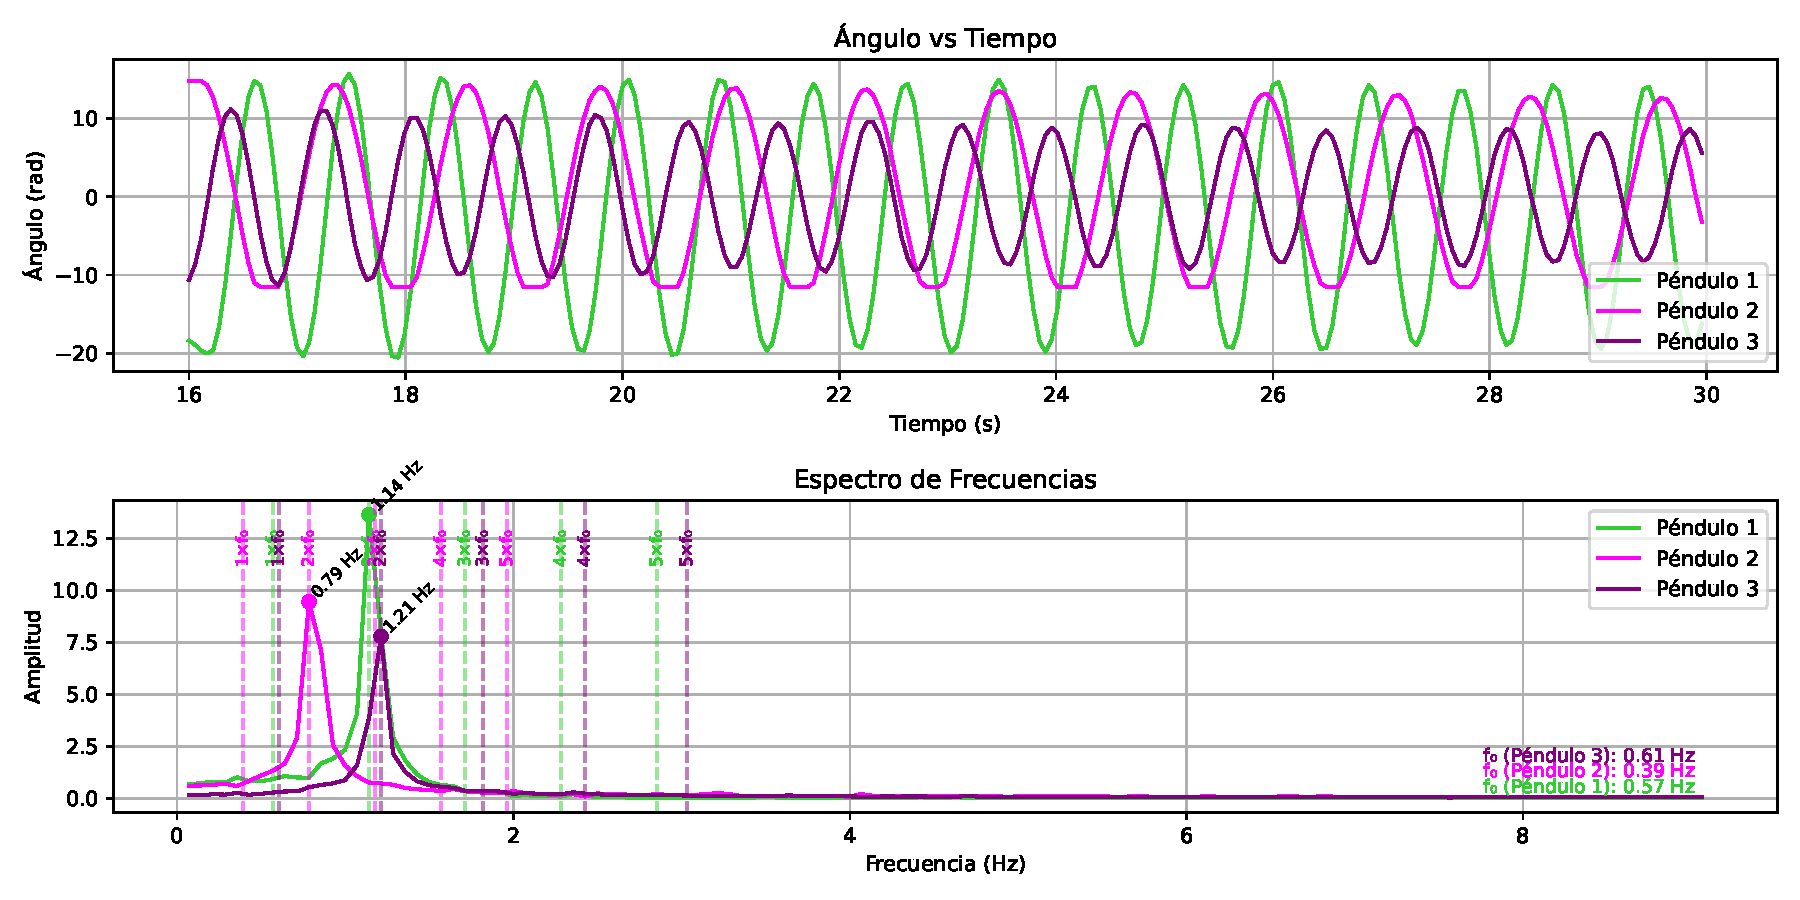
\includegraphics[width=0.8\linewidth]{./Figures/111_11_filtrado.pdf}
  \caption{Evoluci\'on temporal $\theta_i(t)$ y espectro FFT.
  Configuraci\'on 1-1, CI (111).}
  \label{fig:111-11}
\end{figure}

\begin{figure}[htbp!]
  \centering
  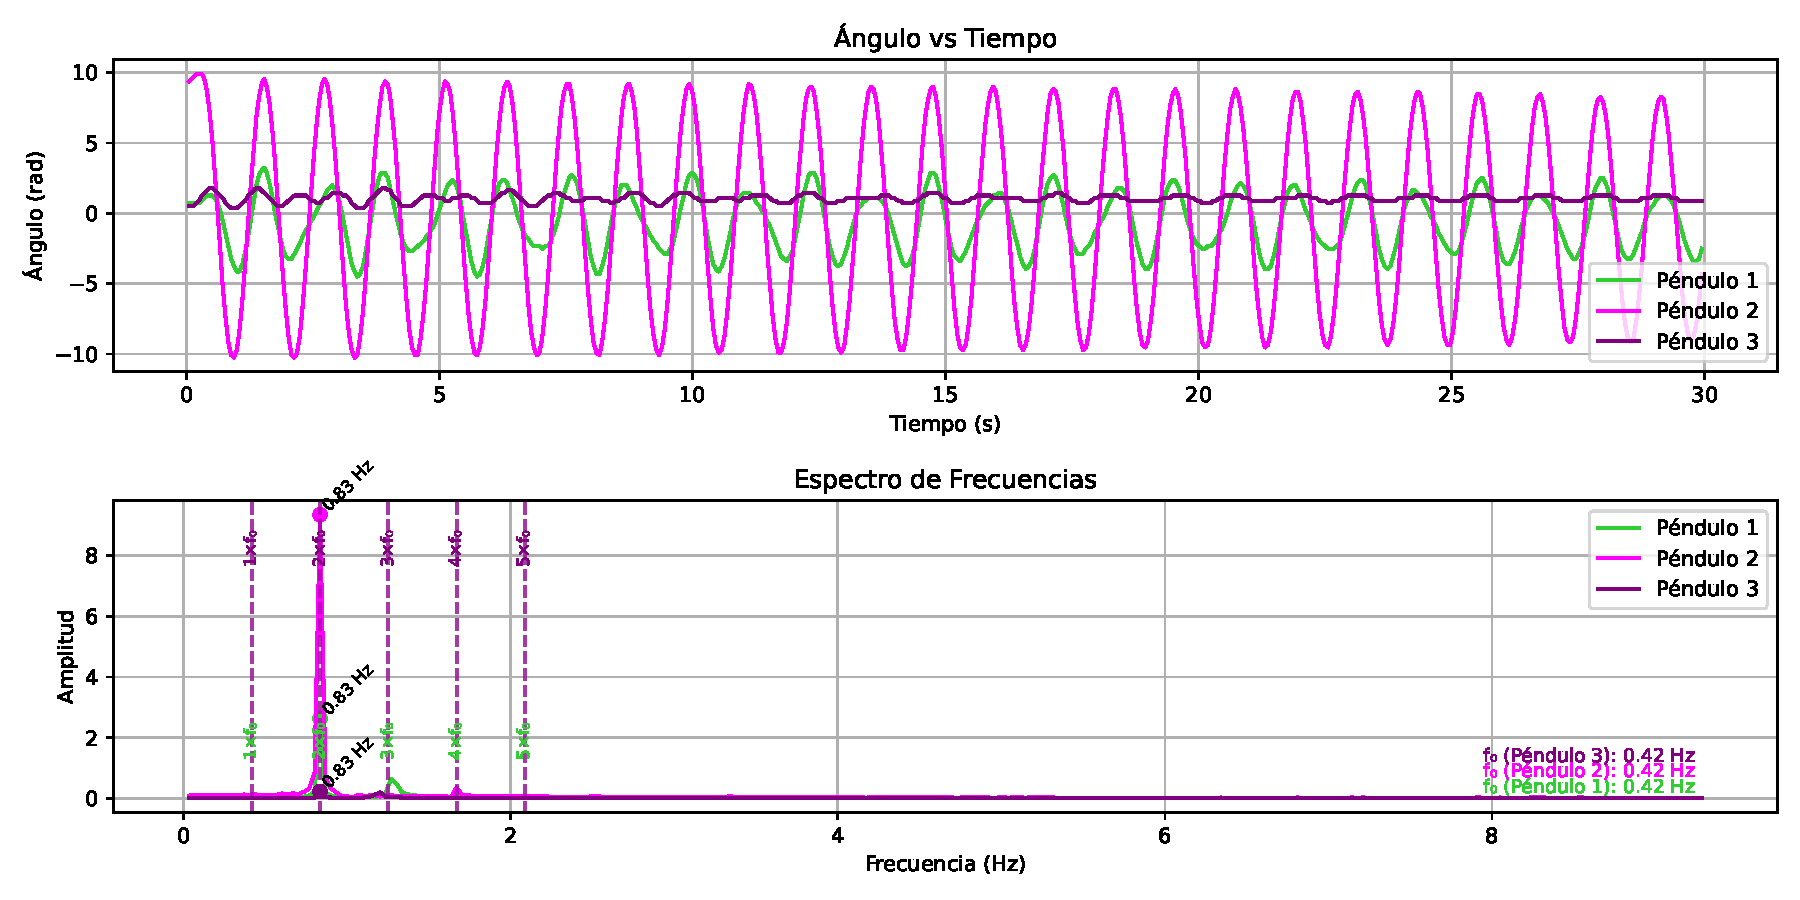
\includegraphics[width=0.8\linewidth]{./Figures/010_15_filtrado.pdf}
  \caption{Evoluci\'on temporal $\theta_i(t)$ y espectro FFT.
  Configuraci\'on 5-1, CI (010).}
  \label{fig:010-51}
\end{figure}

\begin{figure}[htbp!]
    \centering
    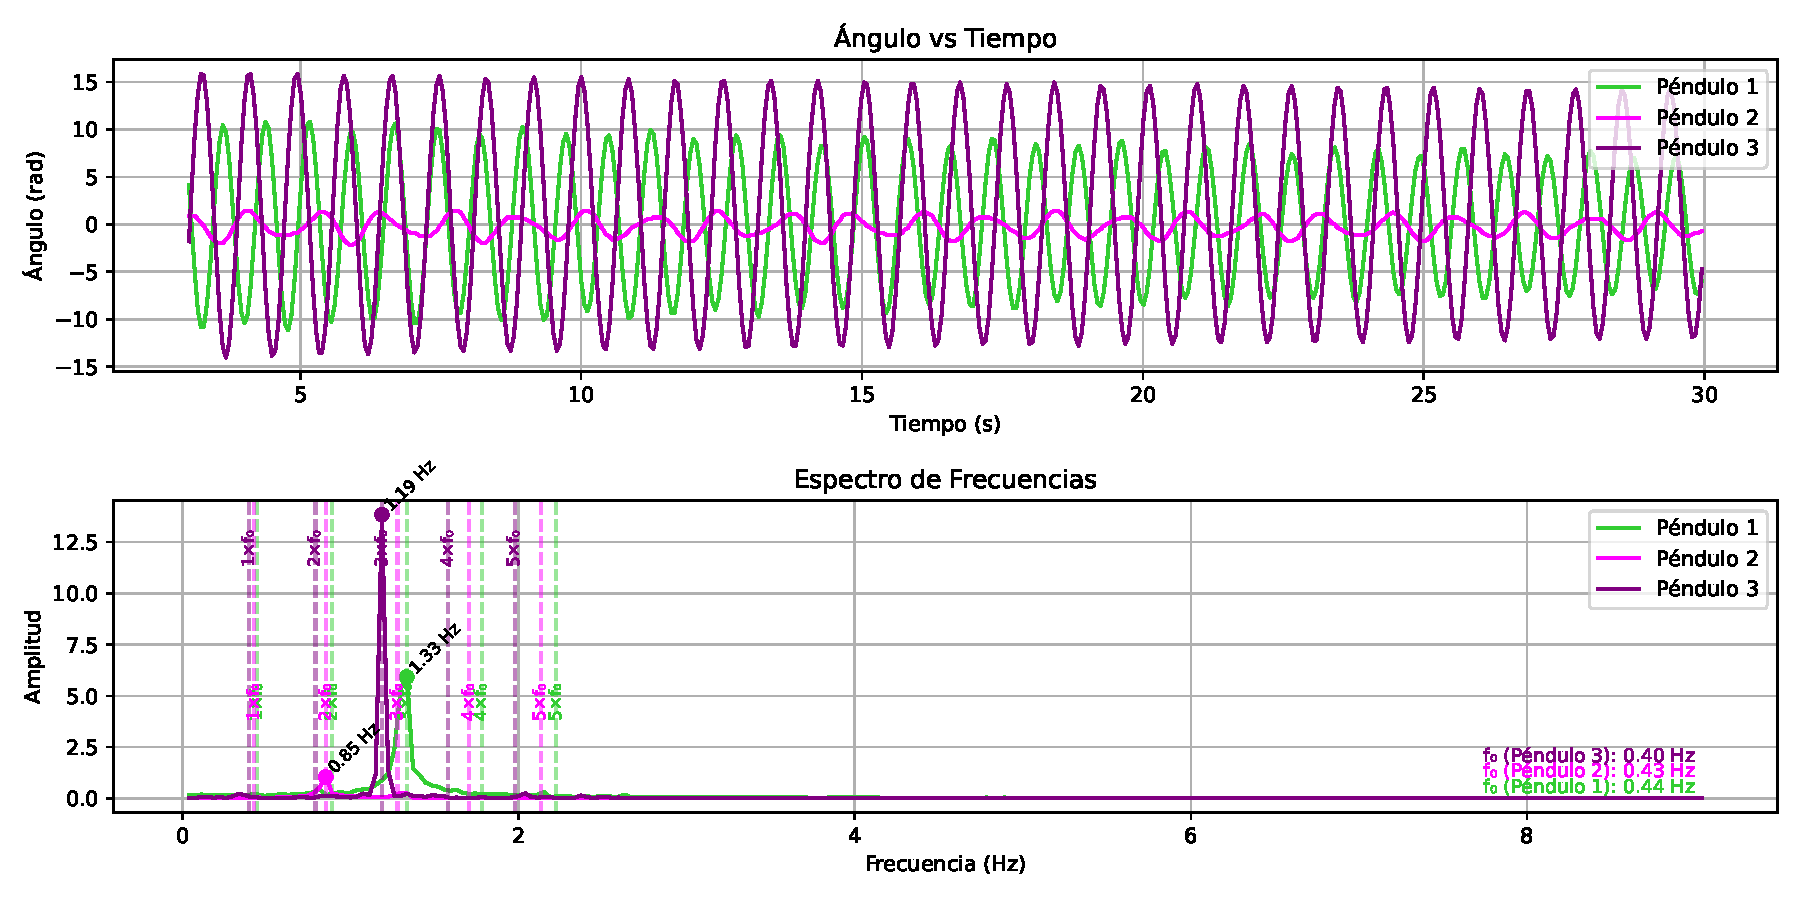
\includegraphics[width=0.8\linewidth]{./Figures/101_16_filtrado.pdf}
    \caption{Evoluci\'on temporal $\theta_i(t)$ y espectro FFT.
        Configuraci\'on 6-1, CI (101).}
    \label{fig:101-61}
\end{figure}

\begin{figure}[htbp!]
    \centering
    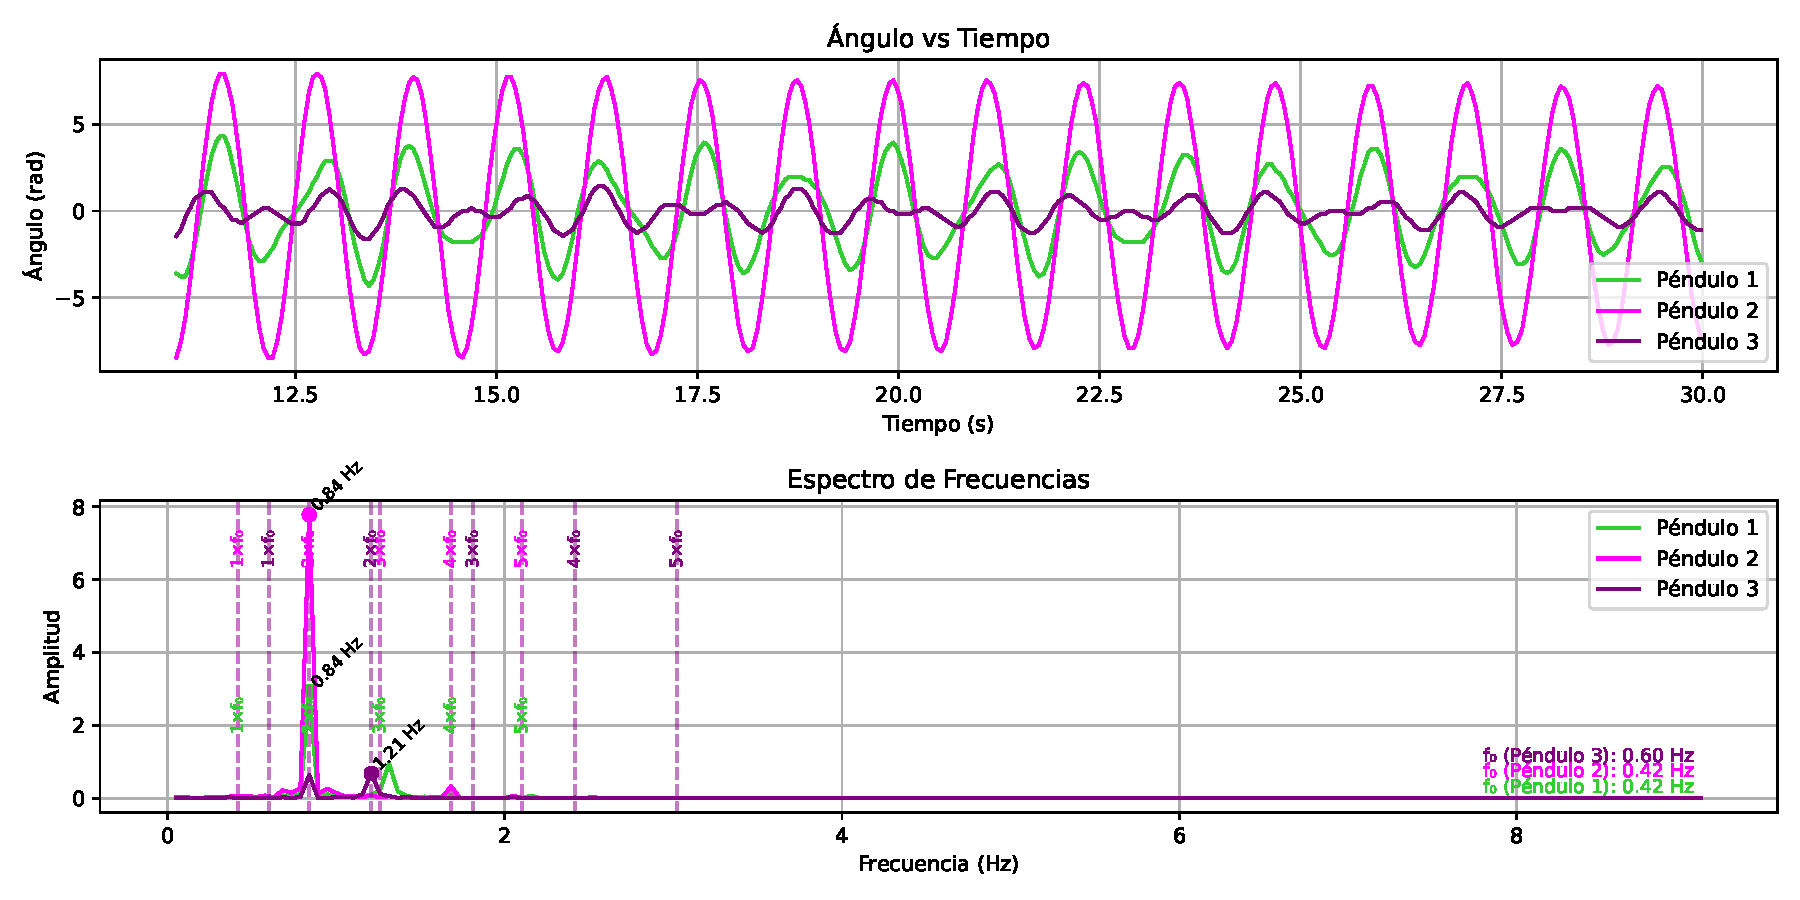
\includegraphics[width=0.8\linewidth]{./Figures/010_26_filtrado.pdf}
    \caption{Evoluci\'on temporal $\theta_i(t)$ y espectro FFT.
        Configuraci\'on 6-2, CI (010).}
    \label{fig:010-62}
\end{figure}

\begin{figure}[htbp!]
    \centering
    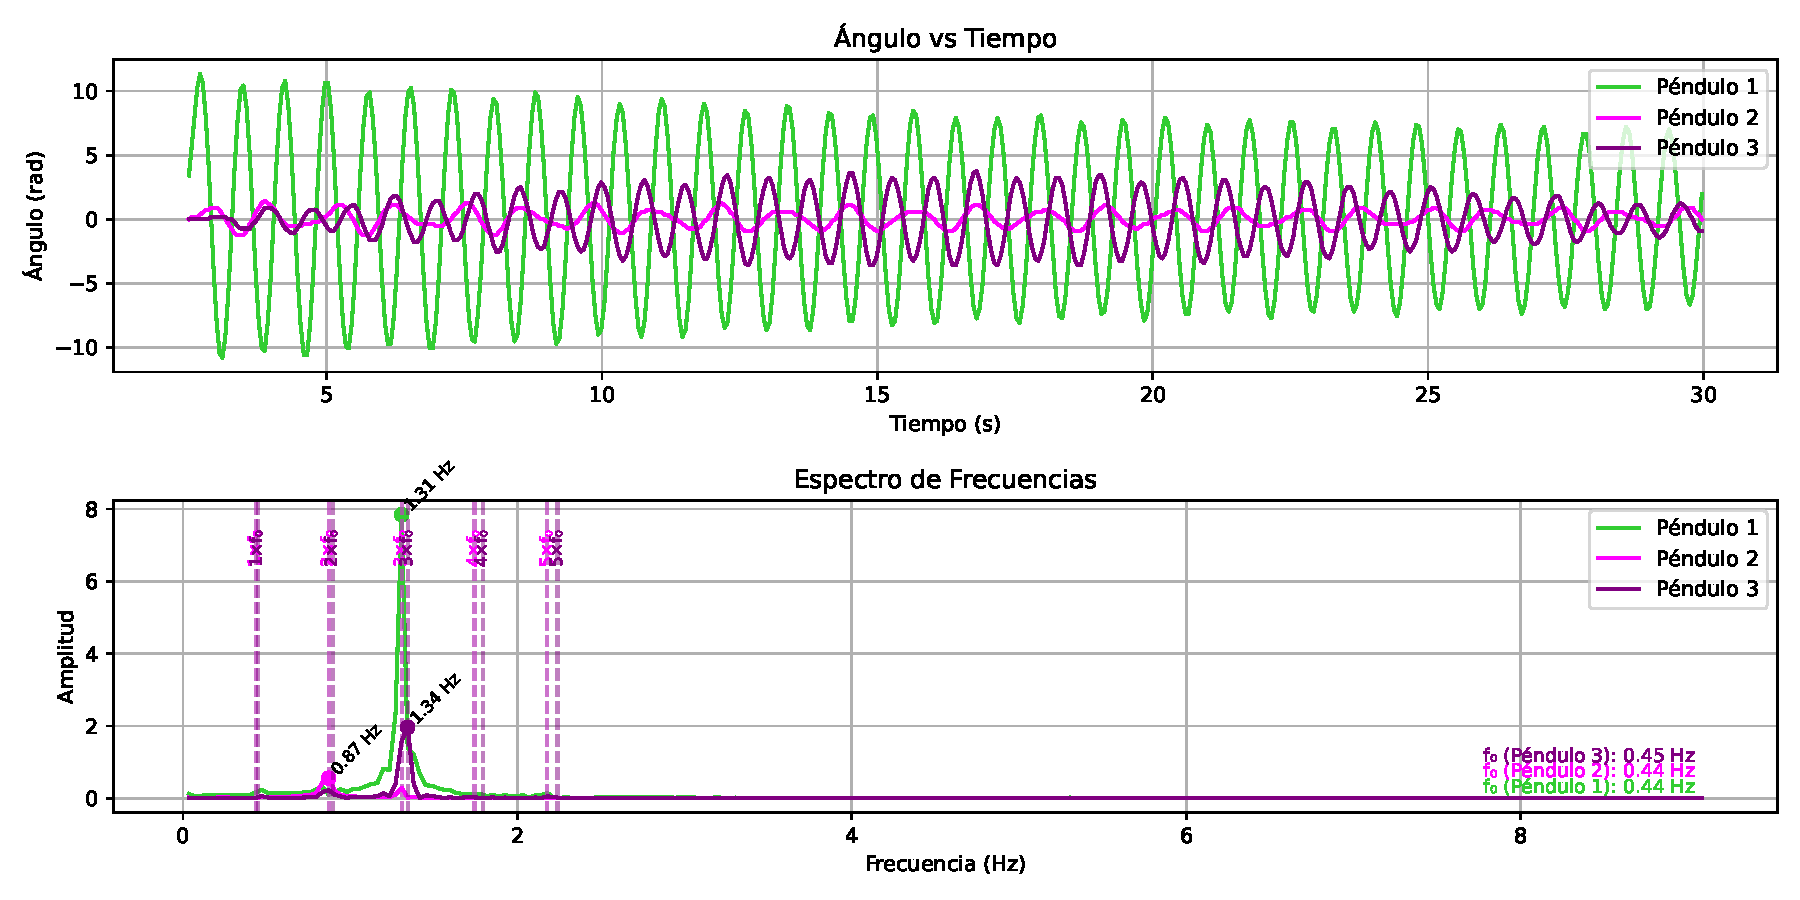
\includegraphics[width=0.8\linewidth]{./Figures/001_66_filtrado.pdf}
    \caption{Evoluci\'on temporal $\theta_i(t)$ y espectro FFT.
        Configuraci\'on 6-6, CI (100).}
    \label{fig:100-66}
\end{figure}

\begin{figure}[htbp!]
    \centering
    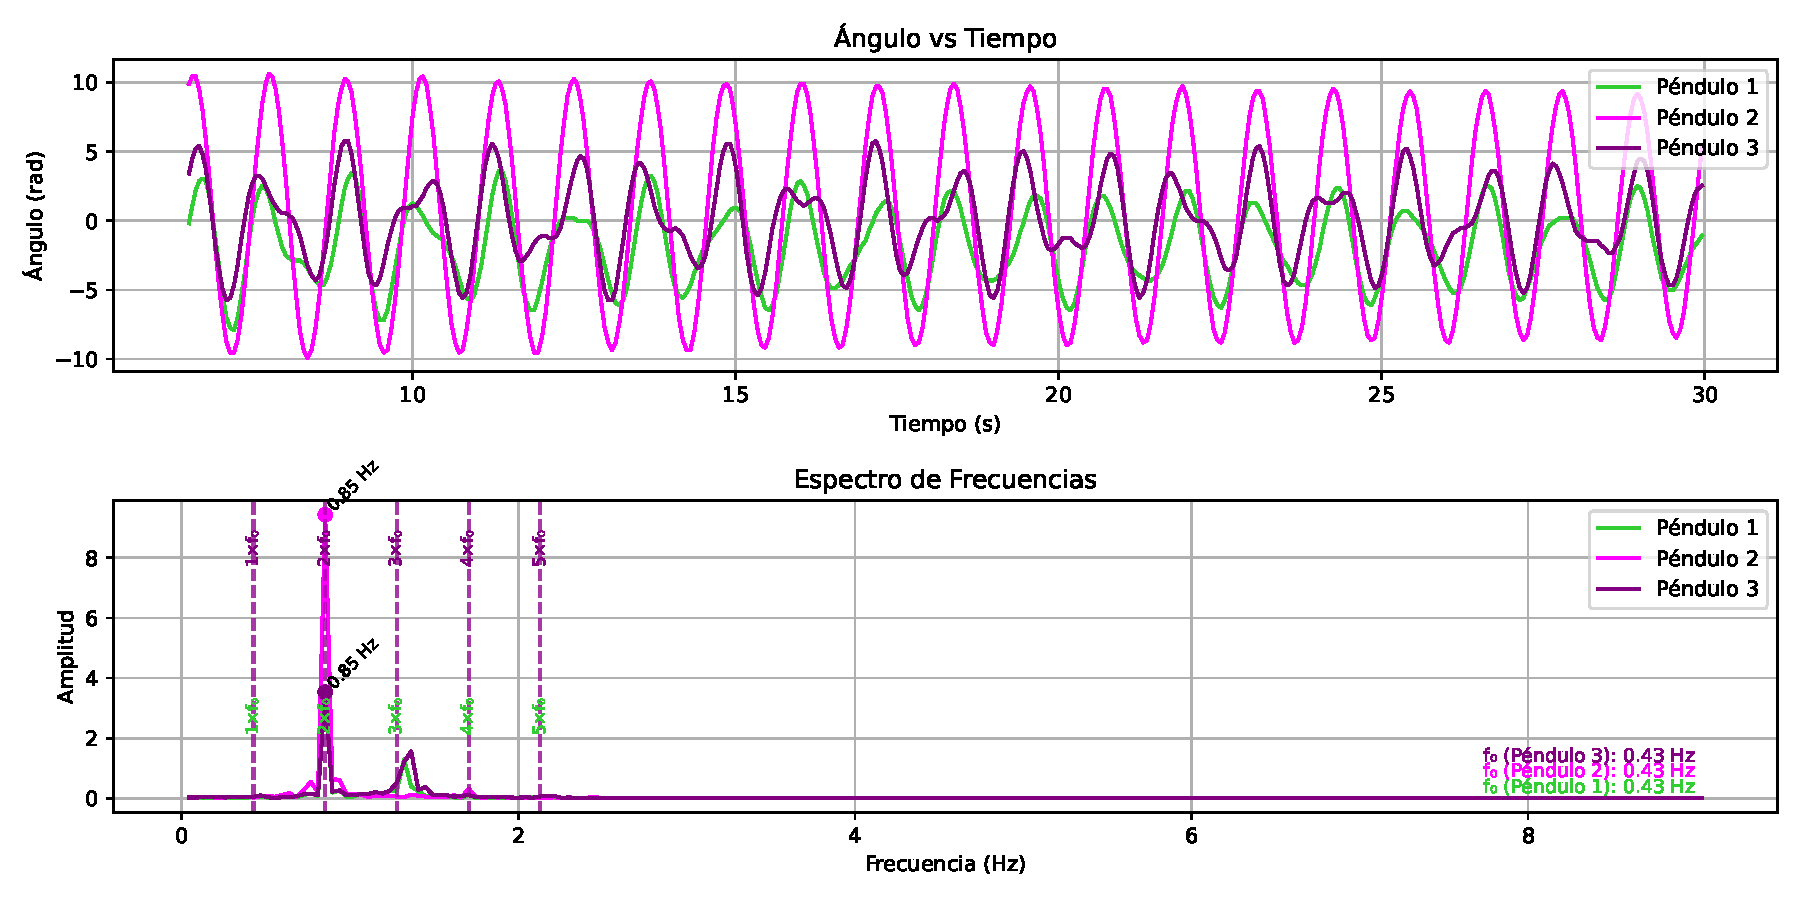
\includegraphics[width=0.8\linewidth]{./Figures/010_66_filtrado.pdf}
    \caption{Evoluci\'on temporal $\theta_i(t)$ y espectro FFT.
        Configuraci\'on 6-6, CI (010).}
    \label{fig:010-66}
\end{figure}

\textbf{An\'alisis de casos espec\'ificos:}

\textbf{\Cref{fig:111-11} (Config. 1-1, CI (111)):}
\begin{itemize}
  \item Cada p\'endulo exhibe un pico de frecuencia principal distintivo en su
    FFT; no comparten una \'unica frecuencia dominante com\'un.
  \item Picos espectrales relativamente anchos: sugiere duraci\'on limitada
    de coherencia o amortiguamiento significativo.
  \item Amortiguamiento esperado: debido a interacciones (acoplamiento,
    fricci\'on) y complejidad del movimiento (laterales desfasados
    respecto al central).
  \item P\'endulo 2: comportamiento temporal con modulaciones en amplitud,
    no arm\'onico simple.
\end{itemize}

\textbf{\Cref{fig:010-51} (Config. 5-1, CI (010)):}
\begin{itemize}
  \item Picos espectrales m\'as definidos y estrechos: comportamiento m\'as
    regular, menos amortiguado para frecuencias dominantes.
  \item Los tres p\'endulos comparten la misma frecuencia principal (reafirma
    tendencia para CI (010)).
  \item Componentes espectrales secundarias comunes, con diferentes
    amplitudes relativas entre p\'endulos.
  \item P\'endulo 3: menor amplitud en componentes espectrales (posiblemente
    menor eficiencia en transmisi\'on de energ\'ia por geometr\'ia de
    acople).
  \item Evoluci\'on temporal m\'as estable y coherente; disminuci\'on gradual
    de amplitudes (amortiguamiento residual).
\end{itemize}

\textbf{\Cref{fig:101-61} (Config. 6-1, CI (101)):}
\begin{itemize}
  \item An\'alisis espectral revela tres picos de frecuencia principales
    distintos (sugiere excitaci\'on de m\'ultiples modos normales).
  \item P\'endulo 3: mayor amplitud en su frecuencia principal y pico
    espectral m\'as estrecho comparado con P1 (relacionado con
    naturaleza del acoplamiento y excitaci\'on inicial de P3).
  \item P\'endulo 2: oscilaciones de amplitud muy reducida (consistente con
    modo normal donde laterales se mueven desfasados y P2 tiene
    participaci\'on m\'inima).
  \item Evoluci\'on temporal: intercambio de energ\'ia entre P1 y P3
    (pulsaciones/batidos), esperado si frecuencias de modos son cercanas
    y hay transferencia de energ\'ia.
\end{itemize}

\textbf{\Cref{fig:010-62} (Config. 6-2, CI (010)):}
\begin{itemize}
  \item P\'endulo 2 (espectro): frecuencia principal con amplitud prominente y
    pico estrecho. Componente secundaria a aprox. $4 f_P$.
    Comportamiento temporal similar a M.A.S.
  \item P\'endulo 1 (espectro): comparte $f_P$ de P2. Otro pico significativo
    a frecuencia $> 3 f_P$. Movimiento no estrictamente M.A.S.,
    pero con clara periodicidad.
  \item P\'endulo 3 (espectro): dos picos con amplitudes comparables,
    frecuencias corresponden aprox. con valores te\'oricos esperados
    (\qty{0.83}{\Hz} y \qty{1.2}{\Hz}). Amplitudes bajas, oscilaci\'on
    de escasa magnitud.
\end{itemize}

\textbf{\Cref{fig:100-66} (Config. 6-6, CI (100)):}
\begin{itemize}
  \item Geometr\'ia de acople facilita transmisi\'on efectiva de energ\'ia.
  \item An\'alisis espectral: los tres p\'endulos comparten componentes de
    frecuencia en mismas ubicaciones espectrales.
  \item P1 y P3 comparten frecuencia principal com\'un (m\'as alta).
  \item P2 tiene su propia $f_P$ (menor), pero exhibe picos secundarios en
    frecuencias donde P1 y P3 oscilan predominantemente (participa en
    modos de mayor frecuencia).
  \item Comportamiento (todos oscilan significativamente) distingue esta
    combinaci\'on, resaltando papel determinante de posici\'on de acoples.
\end{itemize}

\section{Conclusiones}

Se ha investigado con \'exito el comportamiento din\'amico
de un sistema de tres p\'endulos acoplados, confirmando la validez y
aplicabilidad de la aproximaci\'on de peque\~nas oscilaciones para
describir su movimiento. Mediante un montaje experimental controlado y
el an\'alisis de datos con la Transformada R\'apida de Fourier (FFT),
se lograron identificar las frecuencias de los modos normales de
oscilaci\'on, cumpliendo el objetivo principal de visualizar y
cuantificar estos patrones fundamentales en un sistema cl\'asico.

Los resultados experimentales mostraron una fenomenolog\'ia de
oscilaciones acopladas, donde la frecuencia dominante de cada p\'endulo
var\'ia seg\'un la configuraci\'on de los resortes y las condiciones
iniciales aplicadas. El p\'endulo central (el m\'as largo) exhibi\'o
una frecuencia notablemente consistente alrededor de \qty{0.844}{\Hz}.
Por su parte, los p\'endulos laterales a menudo presentaron una
dualidad de frecuencias predominantes, lo que sugiere la excitaci\'on
simult\'anea de m\'ultiples modos. La comparaci\'on cuantitativa revel\'o
que el modelo te\'orico linealizado predice estas frecuencias con
una precisi\'on notable, con errores relativos porcentuales que en
la mayor\'ia de los casos se sit\'uan entre \qty{0.036}{\percent} y
\qty{2.509}{\percent}. Esta estrecha concordancia valida la capacidad
del marco te\'orico para describir con fiabilidad el sistema
experimental.

El an\'alisis tambi\'en puso de manifiesto el papel cr\'itico de la
geometr\'ia de acoplamiento. Se observ\'o c\'omo la posici\'on de los
resortes influye en la rigidez efectiva angular, determinando la
transmisi\'on de energ\'ia y las frecuencias de los modos excitados.
Particularmente, ciertas configuraciones y condiciones iniciales
favorecieron la oscilaci\'on de los tres p\'endulos a una misma
frecuencia, mientras que otras revelaron complejas interacciones de
energ\'ia, como el fen\'omeno de pulsaciones entre los p\'endulos
laterales.

Sin embargo, el estudio tambi\'en identific\'o una frecuencia
experimental an\'omala excepcionalmente baja (\qty{0.0021}{\Hz}) en
una configuraci\'on espec\'ifica, la cual no encuentra una
contraparte directa en el modelo te\'orico linealizado. Esta
discrepancia sugiere la posible influencia de factores no incluidos
en el modelo ideal, como efectos no lineales para desplazamientos
angulares mayores, o la presencia de amortiguamiento diferencial en
el sistema.

Como trabajo futuro, ser\'ia valioso: incorporar t\'erminos de
amortiguamiento en el modelo te\'orico para una comparaci\'on m\'as
precisa con los datos experimentales, realizar un an\'alisis
cuantitativo detallado de los vectores propios (formas modales) para
relacionar directamente los patrones de movimiento observados con los
modos te\'oricos, y explorar el comportamiento del sistema bajo
condiciones que acent\'uen las no linealidades, con el fin de entender
fen\'omenos como la frecuencia an\'omala observada.


\bibliography{ref}

\end{document}
